\documentclass[a4paper,12pt]{article}

% Paquetes necesarios
\usepackage[utf8]{inputenc}   % Codificación UTF-8
\usepackage{fontspec} % Paquete para manejar fuentes específicas
\usepackage[spanish]{babel}
\usepackage[style=apa, backend=biber]{biblatex}
\usepackage{geometry}         % Configuración de márgenes
\usepackage{graphicx}
\usepackage{setspace}         % Configuración de interlineado
\usepackage{fancyhdr}         % Configuración de encabezados y pie de página
\usepackage{biblatex}
\usepackage{hyperref}

\setmainfont{Arial}   % Configura Arial como la fuente principal
\geometry{
    top=2.5cm,
    bottom=2.5cm,
    left=4cm,
    right=2.5cm
}
\pagestyle{fancy}
% Configuración del interlineado y espacio entre párrafos
\onehalfspacing            % Interlineado de 1.5
% Configuración del pie de página
\fancyhf{}
\fancyfoot[R]{\thepage}    % Número de página en la esquina inferior derecha
\fancypagestyle{plain}{
    \fancyhf{}
    \fancyfoot[R]{\thepage}
}

\addbibresource{bibliography.bib} % Archivo .bib con las referencias


\begin{document}

% Incluir la portada
% Archivo: portada.tex
\begin{titlepage}
    \begin{center}
        % Logo
        
\includegraphics[width=0.8\textwidth]{images/logo_soe.png} \\
        \vspace{1cm}
        % Título de la institución

        {\fontsize{18pt}{10pt}\selectfont\textbf{FACULTAD DE INGENIERÍA EN CIENCIAS DE LA COMPUTACIÓN Y TELECOMUNICACIONES}} \\
        \vspace{2cm}
        {\fontsize{18pt}{5pt}\selectfont\textbf{UNIDAD DE POSTGRADO SCHOOL OF ENGINEERING}} \\
        \vspace{0.5cm}
        
        % Nombre de la maestría
        \vspace{0.5cm}
        {\fontsize{20pt}{5pt}\selectfont\textbf{MONOGRAFIA}} \\
        \vspace{1cm}
        
        % Título del trabajo
        {\fontsize{16pt}{5pt}\selectfont\textbf{Anáslis de programación multiplataforma para abaratar costos en el desarrollo de aplicaciones móbiles}} \\
        \vspace{1cm}
        
        \vspace{2cm}
        {\fontsize{14pt}{22pt}\selectfont\textbf{Ing. Joel Gabriel Torrejón Méndez}} \\
        
        % Ciudad y fecha
        \vfill
        \textbf{Santa Cruz, Bolivia} \\
    \end{center}
\end{titlepage}
     % Reemplaza con % Archivo: portada.tex
\begin{titlepage}
    \begin{center}
        {\fontsize{15pt}{10pt}\selectfont\textbf{UNIVERSIDAD AUTÓNOMA "GABRIEL RENE MORENO"}} \\
        {\fontsize{15pt}{10pt}\selectfont\textbf{FACULTAD DE INGENIERÍA EN CIENCIAS DE LA COMPUTACIÓN Y TELECOMUNICACIONES}} \\
        \vspace{1cm}
        % Logo
        
\includegraphics[width=0.8\textwidth]{images/logo_soe.png} \\
        
        % Título de la institución
        {\fontsize{15pt}{10pt}\selectfont\textbf{MAESTRÍA EN CIENCIA DE DATOS E INTELIGENCIA ARTIFICIAL}} \\

        % Título del trabajo
        \vspace{1cm}
        {\fontsize{15pt}{5pt}\selectfont\textbf{Implementar un Chatbot Semántico Multiperfil para Acceso Inteligente a Documentación Técnica y de Negocio en Plataformas Confluence del Sector Aeronáutico en Airnguru S.A. para la Gestión 2025}} \\
        \vspace{1cm}
        
        \vspace{2cm}
        \begin{flushright}
        {\fontsize{14pt}{22pt}\selectfont\textbf{Autor}} \\
        {\fontsize{14pt}{22pt}\selectfont{Ing. Darlyn Bravo Peña}} \\
        \end{flushright}
        
        
        
        % Ciudad y fecha
        \vfill
        \textbf{Santa Cruz, Bolivia} \\
    \end{center}
    \end{titlepage}
     si prefieres que se trate como una sección independiente

% Table of contents
\newpage
\tableofcontents
% \listoffigures

\section{Introducción}

La programación híbrida en aplicaciones móviles es una estrategia ideal para desarrollar
soluciones multiplataforma con un presupuesto reducido. Este enfoque permite crear una
única base de código utilizando tecnologías web como HTML, CSS y JavaScript, que luego
se empaqueta en un contenedor nativo para ejecutarse en dispositivos Android e iOS.
Frameworks como Ionic, React Native o Flutter optimizan el proceso, permitiendo un
desarrollo ágil y reduciendo significativamente los costos y tiempos asociados con la
creación de apps separadas para cada plataforma.\\

Además de abaratar costos iniciales, las aplicaciones híbridas simplifican el mantenimiento
y las actualizaciones, ya que los cambios se realizan sobre un solo código y se reflejan en
todas las plataformas. Aunque pueden tener limitaciones en cuanto al rendimiento para
aplicaciones complejas, son ideales para startups o empresas que necesitan una app
funcional, atractiva y accesible en ambos sistemas operativos sin invertir en desarrolladores
especializados para cada ecosistema.\\

El tema está ubicado en el area 
Ciencias Generales de la Computación Aplicadas y la 
línea Ingeniería de software con un eje de 
Aspectos económicos y de negocio del proceso de desarrollo del software porque los costos
de desarrollo de software son un factor crítico en la toma de decisiones de las empresas.

\section{Antecedentes}

Con el aumento significativo de usuarios de teléfonos móviles en la última
década, casi todas las empresas necesitan desarrollar una aplicación móvil.
Sin embargo, uno de los principales factores que debe tener en cuenta al
desarrollar una aplicación móvil es elegir entre el desarrollo de aplicaciones
móviles nativas o híbridas. \parencite{turing-hibrid-development} \\

Si bien ambas soluciones tienen pros y contras, muchas empresas optan por
las aplicaciones híbridas debido a sus beneficios en términos de presupuesto,
tiempo de comercialización y otros factores. Según un informe de Forbes \parencite{forbes-hibrid-development},
37 de las 50 principales aplicaciones minoristas en Estados Unidos son híbridas.
Además, plataformas populares como Twitter, Instagram, Gmail, Uber, etc.,
utilizan aplicaciones híbridas.\\

En respuesta a estas limitaciones, surgió la programación híbrida como una
alternativa más eficiente y accesible. Este enfoque permite desarrollar
aplicaciones utilizando tecnologías web estándares como HTML, CSS y JavaScript,
combinadas con frameworks que facilitan su integración con funcionalidades
nativas de los dispositivos. Frameworks como Ionic, React Native y Flutter
han demostrado su capacidad para reducir significativamente los costos
y los tiempos de desarrollo, manteniendo una experiencia de usuario satisfactoria.
Este proyecto se centra en analizar cómo la programación híbrida puede ser
una solución viable para optimizar recursos en el desarrollo de aplicaciones
móviles, especialmente en proyectos donde el presupuesto es un factor crítico.

\newpage
\section{Planteamiento del problema}

\subsection{Presentación de las problemáticas}
El desarrollo de aplicaciones móbiles es parte fundamental para las
empresas que buscan expandir su mercado y llegar a un público más amplio. Esto
se debe a que la mayoría de las personas cuentan con un dispositivo móvil y\
acceden a internet a través de él. Sin embargo, el desarrollo de aplicaciones
enfrenta problemáticas como:
\begin{itemize}
    \item \textbf{Mantenimiento de aplicaciones:} Las aplicaciones móviles
        requieren de mantenimiento constante para corregir errores y agregar
        nuevas funcionalidades.
    \item \textbf{Precios elevados:} El desarrollo de aplicaciones móviles
        puede ser costoso, especialmente para pequeñas y medianas empresas.
    \item \textbf{Dificultad para encontrar desarrolladores:} Encontrar
        desarrolladores con experiencia en el desarrollo de aplicaciones
        móviles puede ser complicado.
    \item \textbf{Dificultad para mantenerse actualizado:} El desarrollo de
        aplicaciones móviles requiere de estar al tanto de las últimas
        tecnologías y tendencias.
\end{itemize}

\subsection{Situación problemática}
El desarrollo de aplicaciones móviles es un proceso complejo que requiere de
conocimientos especializados y experiencia. Además, el desarrollo de
aplicaciones móviles puede ser costoso y requiere de mantenimiento constante
para corregir errores y agregar nuevas funcionalidades.\\

Estas limitantes agregan una barrera de entrada en el mercado de aplicaciones
móviles, especialmente para pequeñas y medianas empresas que no cuentan con
los recursos necesarios para desarrollar y mantener una aplicación móvil.

\subsection{Pregunta de investigación}
¿ Como puede el uso de tecnologías de desarrollo multiplataforma ayudar
a simplificar el desarrollo de aplicaciones móviles y abaratar costos?


\newpage
\section{Justificación}

\subsection{Justificación teórica}
El desarrollo de aplicaciones móviles enfrenta desafíos económicos
significativos debido a la necesidad de adaptar las soluciones a diferentes
plataformas, como Android e iOS. El enfoque tradicional de desarrollo nativo
implica la creación de aplicaciones separadas para cada sistema operativo,
utilizando lenguajes y herramientas específicas. Esto no solo incrementa los
costos relacionados con la contratación de desarrolladores especializados, sino
también los tiempos de desarrollo y mantenimiento.\\

En este contexto, el análisis de la programación multiplataforma emerge como
una alternativa teórica y práctica que busca mitigar estos desafíos
económicos.\\


\subsection{Justificación práctica}
Desde una perspectiva práctica, la programación multiplataforma ofrece
una solución directa a los problemas asociados con el desarrollo nativo
al reducir costos, tiempos y complejidad operativa. Empresas y
desarrolladores han adoptado frameworks multiplataforma debido a su
capacidad para generar aplicaciones funcionales y visualmente
atractivas a partir de un único código base.\\

Este enfoque elimina la necesidad de mantener equipos especializados
en múltiples lenguajes y herramientas, disminuyendo significativamente
el gasto en recursos humanos y tecnológicos.

\newpage
\section{Objetivos}

\subsection{Objetivo general}
Analizar el impacto de la programación multiplataforma como estrategia
para reducir costos en el desarrollo de aplicaciones móviles, evaluando
su viabilidad técnica y económica, así como su capacidad para satisfacer
las necesidades de funcionalidad y experiencia de usuario en diferentes
plataformas.

\subsection{Objetivos específicos}
\begin{itemize}
    \item \textbf{Investigar} las características y principios fundamentales de la programación multiplataforma, así como los principales frameworks utilizados en el desarrollo de aplicaciones móviles.
    \item \textbf{Identificar} los factores económicos, técnicos y operativos que influyen en los costos del desarrollo nativo y multiplataforma.
    \item \textbf{Comparar} el rendimiento, la funcionalidad y la experiencia de usuario entre aplicaciones desarrolladas de forma nativa y multiplataforma.
    \item \textbf{Evaluar} la eficiencia del desarrollo multiplataforma en términos de reducción de tiempos, costos de desarrollo y mantenimiento.
    \item \textbf{Proponer} recomendaciones prácticas para la adopción de programación multiplataforma en proyectos móviles, considerando las necesidades específicas de empresas con recursos limitados.
\end{itemize}
\newpage
\section{Alcance}

\subsection{Delimitación o Alcance especial}
El presente estudio se enfocará en analizar el impacto de la programación
multiplataforma en equipos de desarrollo de aplicaciones móviles ubicados
en la ciudad de Santa Cruz. Se tomarán como referencia empresas tecnológicas,
startups y desarrolladores independientes que operan en esta región,
considerando sus necesidades específicas, recursos disponibles y prácticas
actuales de desarrollo.\\

Este enfoque permitirá obtener datos relevantes
y contextuales que reflejen las condiciones económicas y técnicas propias
del sector en Santa Cruz, facilitando la formulación de estrategias
adaptadas a su realidad local.

\subsection{Alcance temporal}
El análisis abarcará el período comprendido desde el año 2015 hasta la
actualidad. Este intervalo se selecciona debido a que marca el auge y
evolución de frameworks de programación multiplataforma, los cuales
han transformado significativamente el desarrollo de aplicaciones móviles.\\

Este enfoque temporal permitirá evaluar cómo ha cambiado la adopción de
estas tecnologías y su impacto en los costos y la eficiencia del
desarrollo en el contexto de los equipos de Santa Cruz.


\newpage
\section{Marco Teórico}

\subsection{Breve esbozo de la evolución e importancia del desarrollo móvil}
El desarrollo móvil ha evolucionado drásticamente desde los años 90 hasta convertirse en
un motor clave de la economía digital actual. En sus inicios, los dispositivos móviles estaban
limitados a funciones básicas, y las pocas aplicaciones disponibles venían preinstaladas por
los fabricantes. Un ejemplo icónico es el juego Snake en los teléfonos Nokia, que marcó el inicio
del interés por los servicios interactivos en dispositivos portátiles.\\

Con el lanzamiento del iPhone en 2007 y la inauguración de la App Store en 2008, el panorama del
desarrollo móvil cambió radicalmente. Por primera vez, los desarrolladores podían distribuir
aplicaciones a una base global de usuarios. Este modelo fue rápidamente adoptado por Android con
su Play Store en el mismo año, lo que dio lugar a una explosión de aplicaciones móviles.
Para 2015, el número de aplicaciones disponibles superaba los 3 millones en ambas plataformas
principales. Gráficamente, se puede observar un crecimiento exponencial en el número de
aplicaciones disponibles desde 2008 hasta la actualidad, destacando el impacto del ecosistema
de tiendas de aplicaciones.\\

En términos de tecnología, el desarrollo inicial de aplicaciones móviles se centró en enfoques
nativos. Los desarrolladores utilizaban Objective-C o Swift para iOS y Java o Kotlin para Android,
logrando un rendimiento óptimo y acceso completo al hardware. Sin embargo, este enfoque implicaba
altos costos y largos tiempos de desarrollo, ya que era necesario escribir y mantener código
separado para cada plataforma.\\

El auge de las tecnologías multiplataforma marcó un punto de inflexión en el desarrollo móvil
a partir de 2015. Frameworks como React Native, lanzado por Facebook, y Flutter, introducido por
Google en 2018, ofrecieron soluciones que permitieron a los desarrolladores escribir un único
código base y desplegarlo en múltiples plataformas. Este avance no solo redujo significativamente
los costos, sino que también acortó los ciclos de desarrollo. Según un estudio de \parencite{statista-hibrid-development}, el 37\% de
los desarrolladores móviles preferían frameworks multiplataforma debido a su
eficiencia y escalabilidad.\\

La importancia del desarrollo móvil en la actualidad es innegable. Se estima que, para 2024,
habrá más de 7.5 mil millones de usuarios de teléfonos móviles en el mundo, lo que convierte
a las aplicaciones móviles en una herramienta esencial para llegar a audiencias masivas. Además,
sectores como el comercio electrónico, la banca y la educación dependen cada vez más de
aplicaciones móviles para interactuar con sus clientes. Un gráfico de la distribución de
usuarios de aplicaciones móviles por sectores muestra cómo el comercio electrónico lidera
con un 24\%, seguido de redes sociales con un 22\% y entretenimiento con un 18\%.\\

Finalmente, la integración de tecnologías emergentes como la inteligencia artificial, el
Internet de las Cosas (IoT) y la realidad aumentada en aplicaciones móviles ha ampliado
aún más su importancia estratégica. Estas innovaciones no solo mejoran la experiencia
del usuario, sino que también generan nuevas oportunidades de negocio, destacando el
papel fundamental del desarrollo móvil en el futuro de la economía global.


\subsection{Barreras de entrada en el mercado de desarrollo móvil}
El desarrollo móvil presenta desafíos significativos para los nuevos actores, especialmente
en términos de costos y complejidad técnica. Estos factores limitan la accesibilidad al mercado,
dificultando que pequeñas empresas o desarrolladores individuales compitan con grandes corporaciones.\\

Una de las principales barreras es la complejidad técnica inherente al desarrollo móvil. Crear
aplicaciones para plataformas como iOS y Android requiere conocimientos avanzados en lenguajes
de programación específicos, como Swift para iOS y Kotlin o Java para Android. Además, los
desarrolladores deben dominar las guías de diseño específicas de cada plataforma, como las Human
Interface Guidelines de Apple o el Material Design de Google. Esto no solo demanda tiempo y
capacitación constante, sino que también encarece el proceso de desarrollo. Por ejemplo, estudios
estiman que el tiempo promedio para desarrollar una aplicación móvil funcional oscila entre 4 y 6 meses,
dependiendo de la complejidad del proyecto.\\

El alto costo inicial del desarrollo es otra barrera crucial. Según encuestas realizadas en 2023,
el costo promedio de desarrollo de una aplicación móvil sencilla se sitúa entre \$40,000 y \$60,000.
Si el proyecto incluye características avanzadas, como integración con sistemas backend o funciones
de realidad aumentada, este costo puede superar los \$150,000. Además, los costos de prueba y
optimización para asegurar la compatibilidad en una amplia gama de dispositivos añaden un gasto significativo.\\

A esto se suma la necesidad de equipos especializados. Mientras que las grandes empresas cuentan con
recursos para contratar equipos multidisciplinarios que abarcan diseño, desarrollo, pruebas y mantenimiento,
las pequeñas empresas y los desarrolladores independientes suelen enfrentarse a la carga de cubrir múltiples
roles. Esto no solo incrementa los tiempos de desarrollo, sino que también eleva el riesgo de errores
o incompatibilidades.\\

En respuesta a estas barreras, han surgido frameworks multiplataforma como React Native y Flutter, que
permiten reducir tanto los costos como el tiempo de desarrollo. Estas herramientas ofrecen la posibilidad
de escribir un único código base que se puede implementar en múltiples plataformas, disminuyendo la carga
técnica y financiera asociada al desarrollo móvil. Sin embargo, la adopción de estas tecnologías requiere
una inversión inicial en capacitación y adaptación, lo que supone un nuevo desafío para quienes ingresan al mercado.\\

En resumen, el desarrollo móvil sigue siendo una oportunidad prometedora, pero las barreras técnicas y
económicas destacan la importancia de soluciones innovadoras para democratizar el acceso a este sector.
Optar por tecnologías eficientes y estrategias optimizadas es esencial para superar estas limitaciones
y competir en un mercado en constante evolución.

\subsection{Reducción de Costos en el Desarrollo Multiplataforma para desarrollo móvil}
El desarrollo móvil ha sido tradicionalmente un proceso costoso y que consume mucho tiempo, especialmente
cuando se requiere el desarrollo de aplicaciones para múltiples plataformas. Cada plataforma (iOS y Android)
tiene sus propias herramientas, lenguajes de programación y guías de diseño, lo que significa que para
alcanzar una audiencia completa, las empresas deben invertir en el desarrollo y mantenimiento de dos versiones
separadas de la misma aplicación. Este enfoque no solo es costoso, sino también ineficiente. Aquí es
donde entra en juego el desarrollo multiplataforma, una solución que ha ganado popularidad al permitir
a los desarrolladores escribir un solo código base que funcione en varias plataformas simultáneamente,
lo que lleva a una reducción significativa en los costos y los tiempos de desarrollo.\\

Una de las principales ventajas de los frameworks multiplataforma, como React Native, Flutter e Ionic,
es que permiten compartir la mayor parte del código entre diferentes plataformas. Esto significa que,
en lugar de desarrollar dos aplicaciones completas, los desarrolladores solo necesitan escribir y
mantener un único conjunto de código, lo que reduce considerablemente el esfuerzo y los costos asociados.
Por ejemplo, en un desarrollo nativo tradicional, se requiere que el equipo de desarrollo mantenga dos
bases de código diferentes, lo que implica no solo un mayor número de programadores, sino también
duplicación de esfuerzos en pruebas y actualizaciones. Con las herramientas multiplataforma, este
costo se reduce considerablemente, ya que el mismo código puede funcionar en iOS, Android e incluso
en la web, sin necesidad de hacer grandes modificaciones.\\

El ahorro en tiempos de desarrollo es igualmente significativo. Tradicionalmente, el desarrollo de
aplicaciones nativas para ambas plataformas podría tomar entre 6 y 12 meses, dependiendo de la
complejidad. Con el uso de frameworks multiplataforma, este tiempo se reduce entre un 30\% y un 50\%, ya
que los desarrolladores solo deben escribir un código base que se adapta a ambos sistemas operativos.
Este ahorro en tiempo no solo reduce los costos, sino que también permite que las aplicaciones lleguen
al mercado más rápido, lo que es crucial para aprovechar oportunidades de negocio en un mercado móvil
en constante cambio.\\

Además de los ahorros directos en desarrollo y tiempo, el uso de herramientas multiplataforma también
optimiza el proceso de mantenimiento. En lugar de tener que actualizar y corregir errores en dos bases
de código separadas, los desarrolladores pueden realizar cambios en un solo lugar, lo que acelera la
implementación de actualizaciones y mejoras. Esto reduce aún más los costos operativos a largo plazo.\\

Los costos de prueba también se ven reducidos, ya que una sola base de código implica un número menor
de pruebas comparado con las aplicaciones nativas, que requieren pruebas en dispositivos separados
para iOS y Android. Con frameworks multiplataforma, el proceso de pruebas se centraliza, lo que
disminuye los costos relacionados con la calidad y validación del producto final.\\

Finalmente, el reducido costo de personal es otra ventaja significativa. Las herramientas multiplataforma
suelen requerir menos especialistas, ya que los desarrolladores que dominan tecnologías como JavaScript,
Dart (en el caso de Flutter) o HTML/CSS pueden trabajar en ambas plataformas, en lugar de requerir equipos
separados especializados en iOS y Android. Esto no solo reduce el costo por contratación, sino que
también mejora la eficiencia del equipo.

\subsection{Aplicaciones, Casos de Estudio y Tendencias futuras en el desarrollo multiplataforma para aplicaciones móviles}
El desarrollo multiplataforma ha demostrado ser una herramienta poderosa en el ámbito de las aplicaciones móviles, permitiendo
a las empresas aprovechar al máximo sus recursos mientras llegan a una audiencia más amplia. Cada vez más empresas adoptan
estas tecnologías debido a su eficiencia en costos y tiempos de desarrollo. En este contexto, explorar algunos casos de estudio
y las tendencias futuras proporciona una visión más clara de cómo se está transformando este campo y hacia dónde se dirige.\\

Uno de los casos más destacados de éxito en el uso de frameworks multiplataforma es Instagram. La popular aplicación de redes
sociales, que originalmente fue desarrollada como una aplicación nativa para iOS, migró a React Native para su versión en
Android. Esta transición permitió a los desarrolladores de Instagram mantener una sola base de código para ambas plataformas,
lo que aceleró las actualizaciones y mejoró la consistencia de la experiencia de usuario. Otro ejemplo es Airbnb, que adoptó
React Native para mejorar la eficiencia del desarrollo en sus aplicaciones móviles. La adopción de esta tecnología permitió
reducir el tiempo de desarrollo en más de un 30\% y optimizar el proceso de mantenimiento a largo plazo.\\

Otro caso relevante es Alibaba, la gigante del comercio electrónico, que también utiliza un enfoque multiplataforma con Flutter,
el framework de Google. La decisión de Alibaba de adoptar Flutter ha permitido a la empresa crear aplicaciones que funcionan no
solo en dispositivos móviles, sino también en escritorios y dispositivos inteligentes, ampliando su alcance y asegurando una
experiencia de usuario coherente en múltiples plataformas.\\

El futuro del desarrollo multiplataforma se perfila con algunas tendencias clave que continuarán evolucionando y ampliando
el alcance de estas tecnologías. Flutter, por ejemplo, ha experimentado un crecimiento explosivo y se espera que se convierta
en una de las herramientas dominantes en el desarrollo móvil. Con Google mejorando continuamente su ecosistema, Flutter
podría dominar tanto el desarrollo para aplicaciones móviles como para aplicaciones de escritorio y web, eliminando
las barreras entre las plataformas y ofreciendo una verdadera solución “escribe una vez, corre en todas partes”.\\

Otra tendencia que se está consolidando es el aumento de la integración de inteligencia artificial y aprendizaje automático
en las aplicaciones móviles. Frameworks como React Native y Flutter ya están comenzando a integrar herramientas que
facilitan la implementación de funciones como el reconocimiento facial, chatbots y recomendaciones personalizadas.
A medida que estas tecnologías se vuelven más accesibles, los desarrolladores podrán crear aplicaciones más inteligentes
y personalizadas, mejorando la experiencia del usuario.

\newpage
\section{Metodología}
\subsection{Enfoque de la investigación}
Este estudio adopta un enfoque cuantitativo para analizar cómo la programación
multiplataforma puede contribuir a la reducción de costos en el desarrollo de
aplicaciones móviles. A través de datos numéricos recopilados de empresas de
desarrollo de software, se compararán los costos asociados con tecnologías
multiplataforma, como Flutter y React Native, frente a las soluciones
nativas tradicionales. Se emplearán métricas como tiempos de desarrollo,
costos de mantenimiento, y cantidad de recursos necesarios para evaluar
objetivamente las diferencias entre ambos enfoques.\\

Para garantizar la validez de los resultados, se realizarán encuestas y estudios
de caso con desarrolladores y empresas del sector. Los datos obtenidos serán
procesados mediante análisis estadísticos para identificar patrones significativos
y establecer correlaciones entre la elección de herramientas multiplataforma
y la optimización de costos. Este enfoque permitirá generar conclusiones
basadas en evidencia objetiva, proporcionando una base sólida para la
toma de decisiones estratégicas en proyectos de desarrollo móvil.

\subsection{Diseño de la investigación}
El diseño metodológico de esta investigación es de tipo no experimental y
transeccional descriptivo, ya que no se manipularán las variables estudiadas,
sino que se observarán y analizarán tal como se presentan en su contexto
natural. El enfoque no experimental permite recolectar información sobre
el impacto de las tecnologías de programación multiplataforma en el
costo del desarrollo de aplicaciones móviles sin alterar las condiciones
existentes, asegurando así que los datos reflejen la realidad del sector.\\

El estudio se desarrollará de forma transeccional, lo que implica la
recopilación de datos en un único momento del tiempo. Este diseño permitirá
describir las características y tendencias actuales en el uso de
tecnologías multiplataforma como Flutter, React Native y Xamarin, así
como su influencia en la optimización de recursos y tiempos de desarrollo.
Los resultados se enfocarán en detallar patrones y correlaciones que
faciliten la comprensión del fenómeno y aporten información relevante
para las decisiones estratégicas en el desarrollo móvil.

\subsection{Población}
La población de este estudio está constituida por profesionales
especializados en el desarrollo de aplicaciones móviles dentro de startups
tecnológicas en Bolivia. En particular, se considera como población
objetivo a los tech leads y desarrolladores senior que participan
directamente en la implementación de tecnologías multiplataforma y
nativas en sus proyectos. Este grupo es clave para proporcionar
información técnica y estratégica relevante sobre los costos y
beneficios de ambas aproximaciones.\\

\subsection{Muestra}
La muestra estará conformada por 30 participantes seleccionados
de manera intencionada, distribuidos entre 3 tech leads y 3
desarrolladores senior de cada una de las 5 startups identificadas
para este estudio. Este tamaño muestral permite garantizar
la diversidad en las perspectivas y experiencias laborales,
al tiempo que facilita un análisis detallado de las prácticas
y decisiones relacionadas con el desarrollo móvil en un entorno
empresarial específico. Esta selección responde a la necesidad
de contar con información representativa del sector y generar
conclusiones aplicables al contexto boliviano.


\subsection{Técnicas e instrumentos}
Para la recolección de datos, se emplearán técnicas cuantitativas que
permitan obtener información objetiva y estandarizada sobre la percepción y
experiencia de los tech leads y desarrolladores senior en el uso de tecnologías
multiplataforma. Las principales técnicas utilizadas serán las encuestas
estructuradas y la revisión documental de proyectos desarrollados por
las startups seleccionadas.\\

El instrumento principal será un cuestionario diseñado específicamente para
este estudio, que incluirá preguntas cerradas y escalas tipo Likert.
Estas preguntas estarán orientadas a recolectar datos sobre costos de
desarrollo, tiempos de implementación, experiencia de usuario, y
facilidad de mantenimiento en proyectos multiplataforma y nativos.
Además, se utilizará una ficha de análisis documental para recopilar
información cuantitativa sobre los proyectos desarrollados por cada
startup, como el número de desarrolladores involucrados, el tiempo
total de desarrollo, y los costos asociados. Los instrumentos serán
validados a través de una prueba piloto aplicada a un grupo reducido
de participantes, asegurando su claridad y pertinencia para alcanzar
los objetivos del estudio.

\subsection{Elaboración del instrumento}
El instrumento principal, un cuestionario estructurado, fue diseñado tomando
en cuenta las necesidades del estudio y las características de la población
objetivo. Se desarrollaron preguntas cerradas y escalas tipo Likert para
garantizar la estandarización de las respuestas y facilitar su análisis
cuantitativo. Las dimensiones incluidas abarcan aspectos como costos,
tiempos de desarrollo, eficiencia en el mantenimiento y experiencia
del usuario en proyectos multiplataforma. Este cuestionario fue
sometido a una prueba piloto para verificar su validez y confiabilidad,
cuyos detalles se presentan en los anexos junto con el formato
final del instrumento.


\newpage
\section{Conclusión}
\subsection{Presentación de resultados}

A continuación presentamos los resultados de la encuesta \textbf{"Uso de tecnologías multiplataforma en el desarrollo de aplica-
ciones móviles."}\\

\textbf{1. ¿Cuál es su cargo en la startup?}

\begin{figure}[h!]
    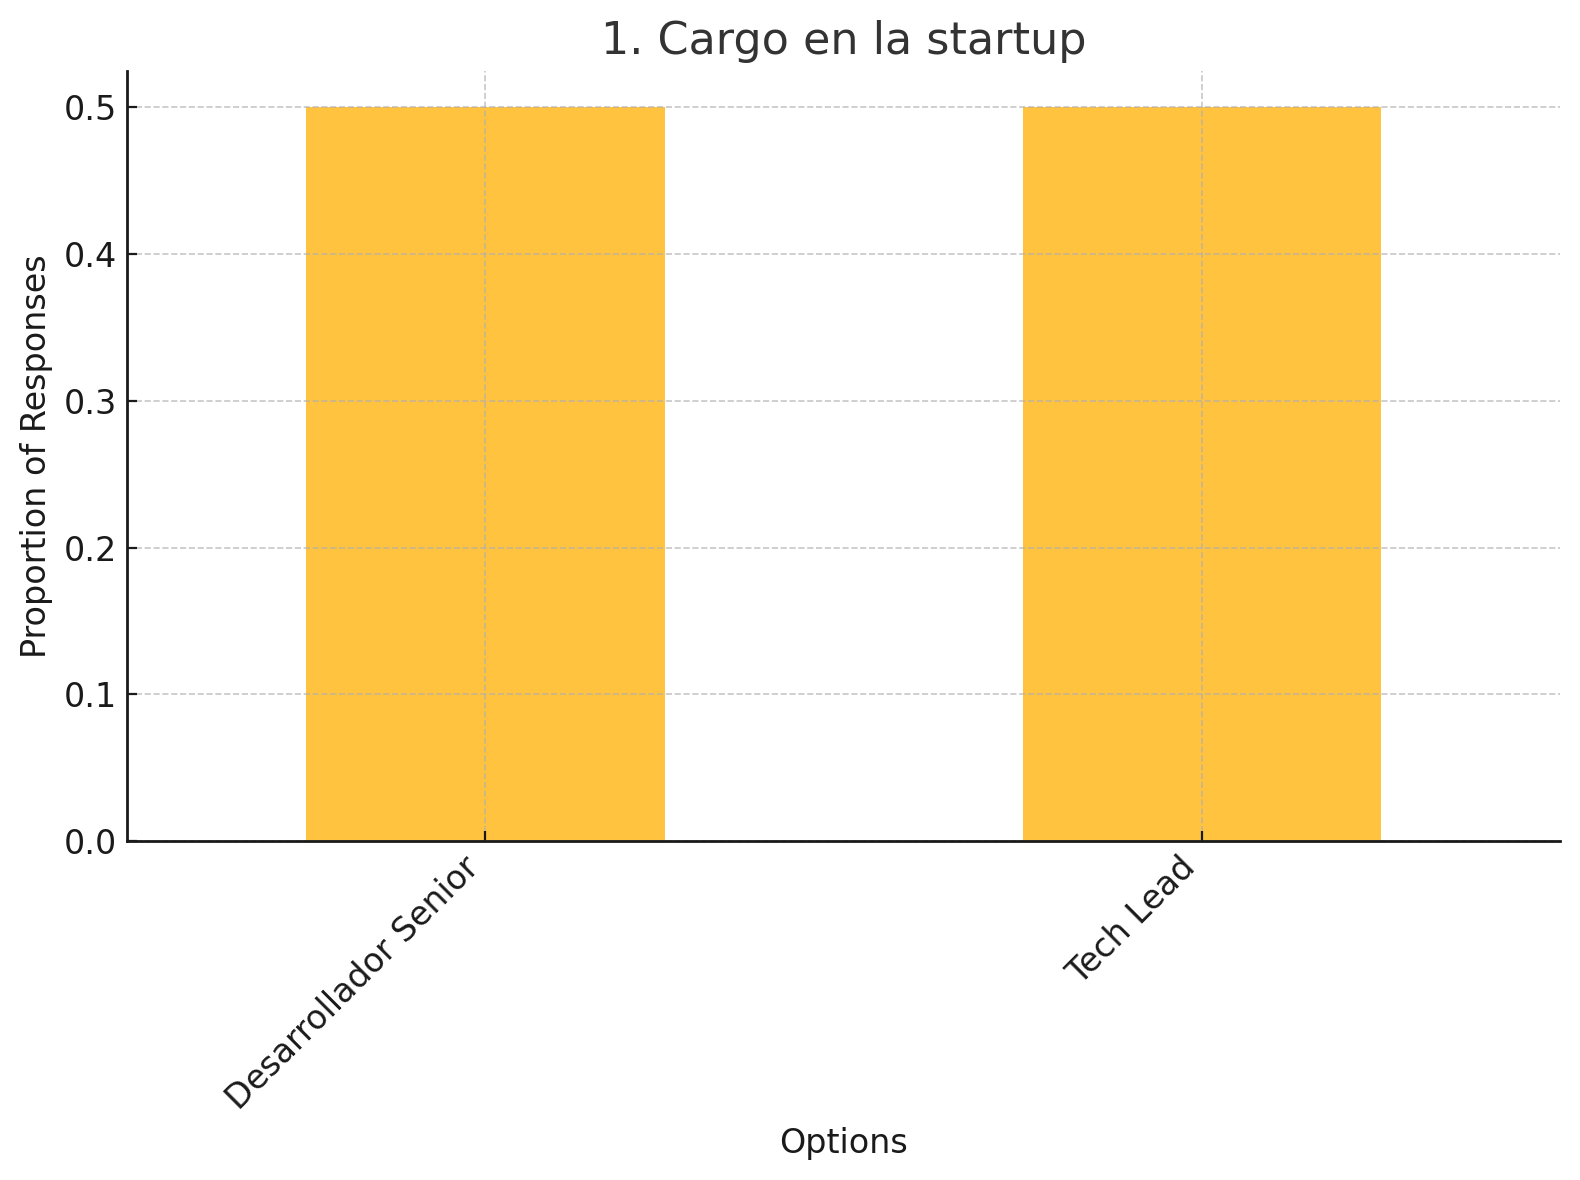
\includegraphics[width=8cm]{images/question1.png}
    \centering
\end{figure}

Conclusión: La mayoría de los encuestados ocupan cargos de Tech Lead o Desarrollador Senior de forma equilibrada, lo que indica que las respuestas reflejan tanto decisiones estratégicas como prácticas en el uso de tecnologías.\\

\textbf{2. ¿Cuántos años de experiencia tiene en el desarrollo de aplicaciones móviles?}

\begin{figure}[h!]
    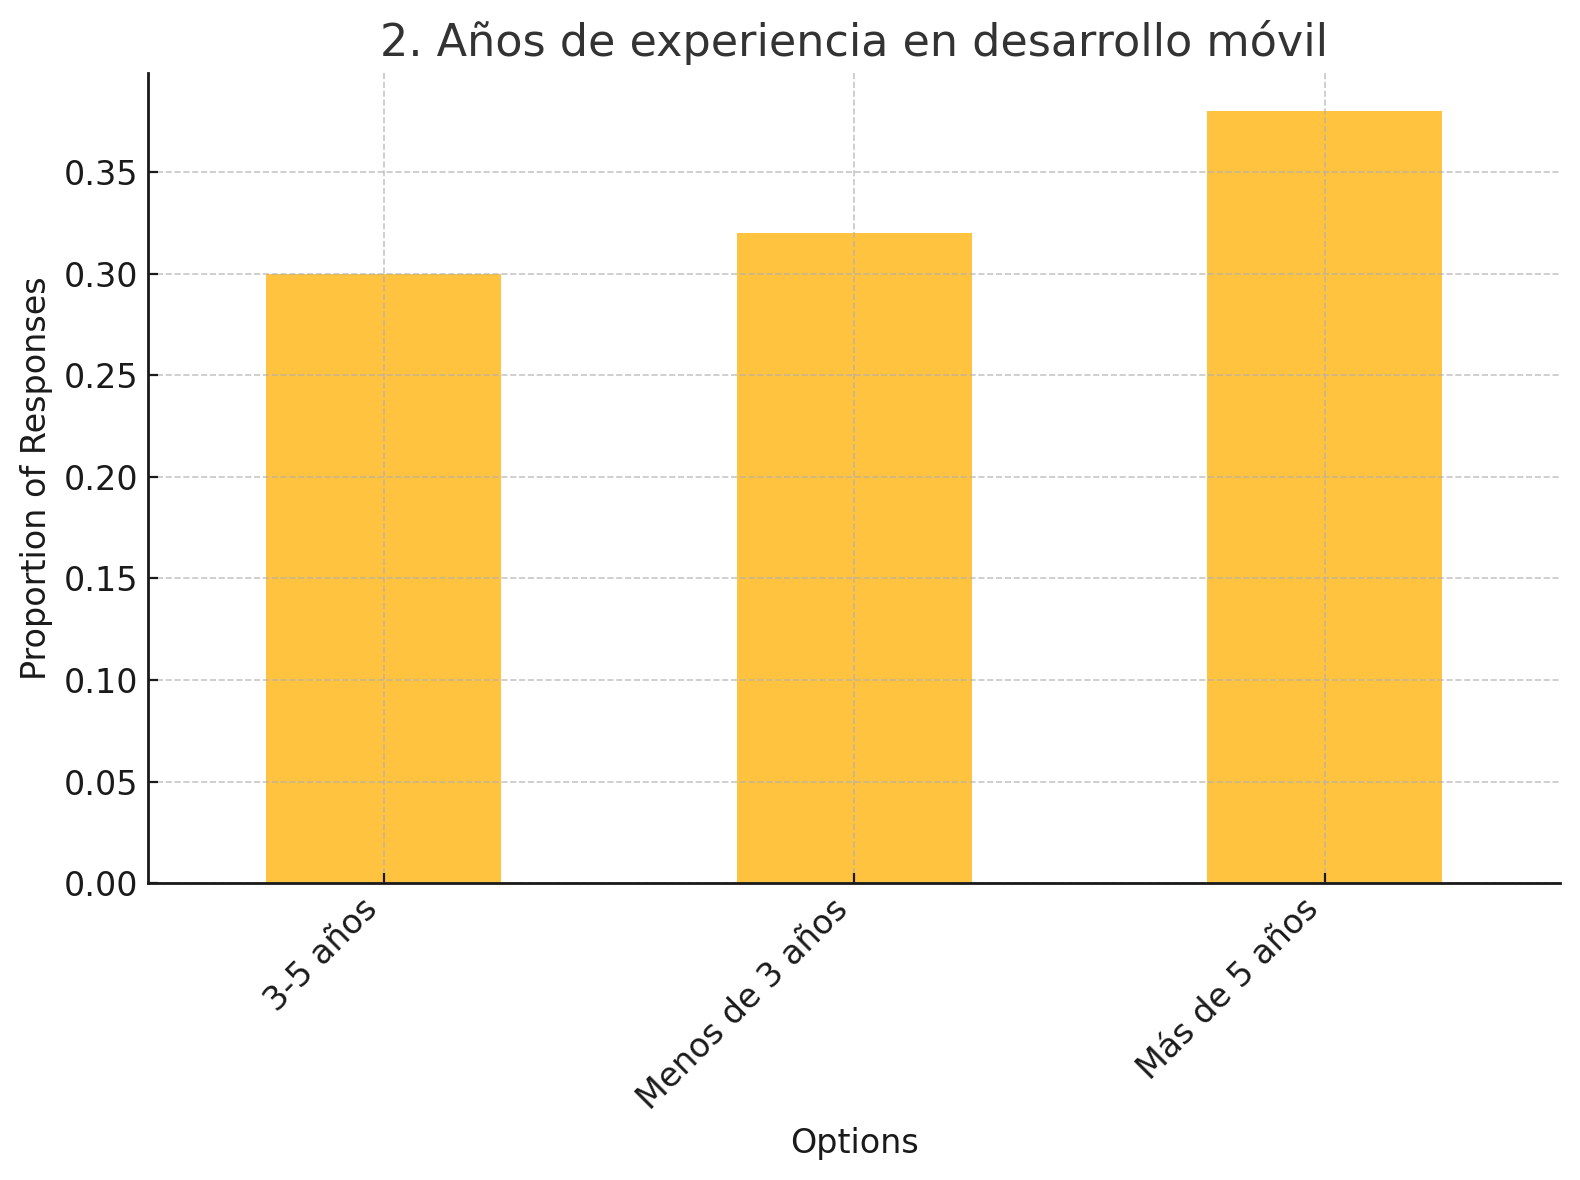
\includegraphics[width=8cm]{images/question2.png}
    \centering
\end{figure}

Conclusión: Predominan los participantes con más de 5 años de experiencia, sugiriendo una perspectiva más informada sobre las ventajas y desventajas de las tecnologías multiplataforma.\\

\textbf{3. ¿Qué tipo de tecnologías utiliza principalmente en su trabajo?}

\begin{figure}[h!]
    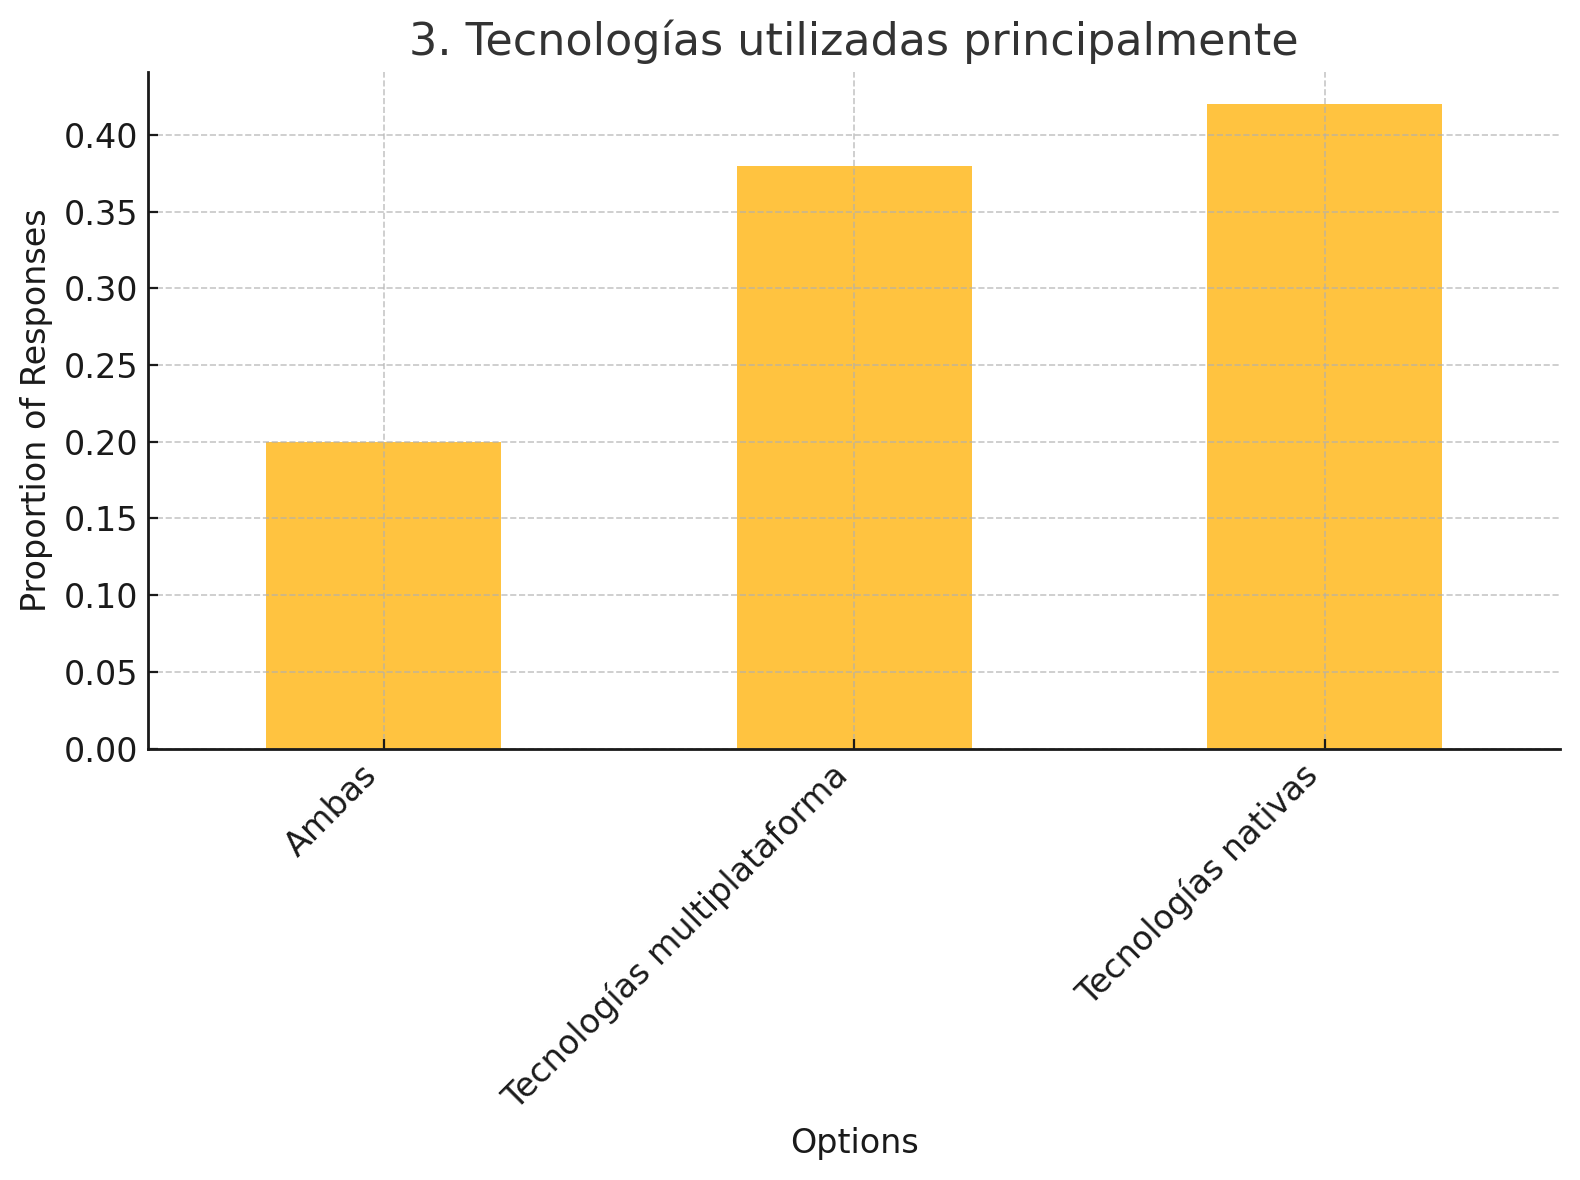
\includegraphics[width=8cm]{images/question3.png}
    \centering
\end{figure}

Conclusión: Un equilibrio entre nativas, multiplataforma y mixto muestra que las empresas adoptan diferentes estrategias dependiendo de sus necesidades específicas.\\

\textbf{4. ¿En qué medida considera que las tecnologías multiplataforma reducen los
costos de desarrollo en comparación con las tecnologías nativas?}

\begin{figure}[h!]
    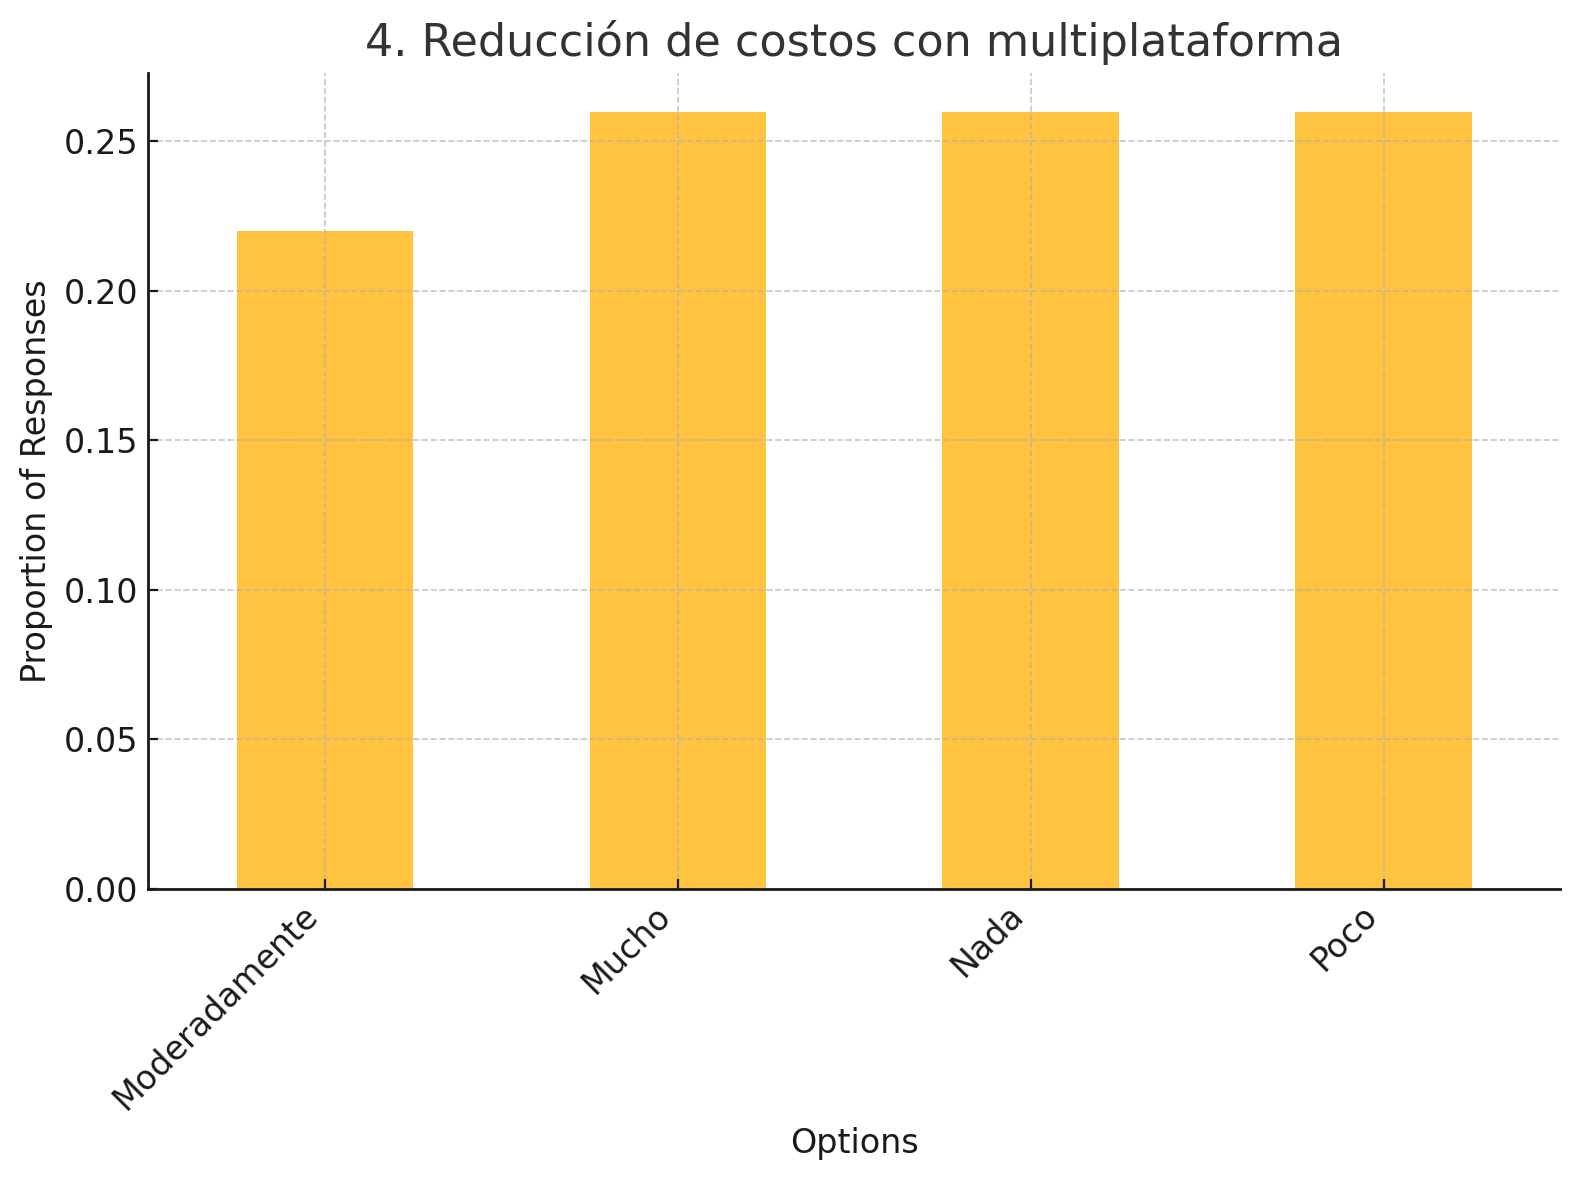
\includegraphics[width=8cm]{images/question4.png}
    \centering
\end{figure}

Conclusión: La mayoría considera que las tecnologías multiplataforma reducen costos moderadamente o mucho, indicando una percepción positiva en términos económicos.\\

\newpage
\textbf{5. Según su experiencia, ¿las tecnologías multiplataforma permiten acortar los
tiempos de desarrollo?}

\begin{figure}[h!]
    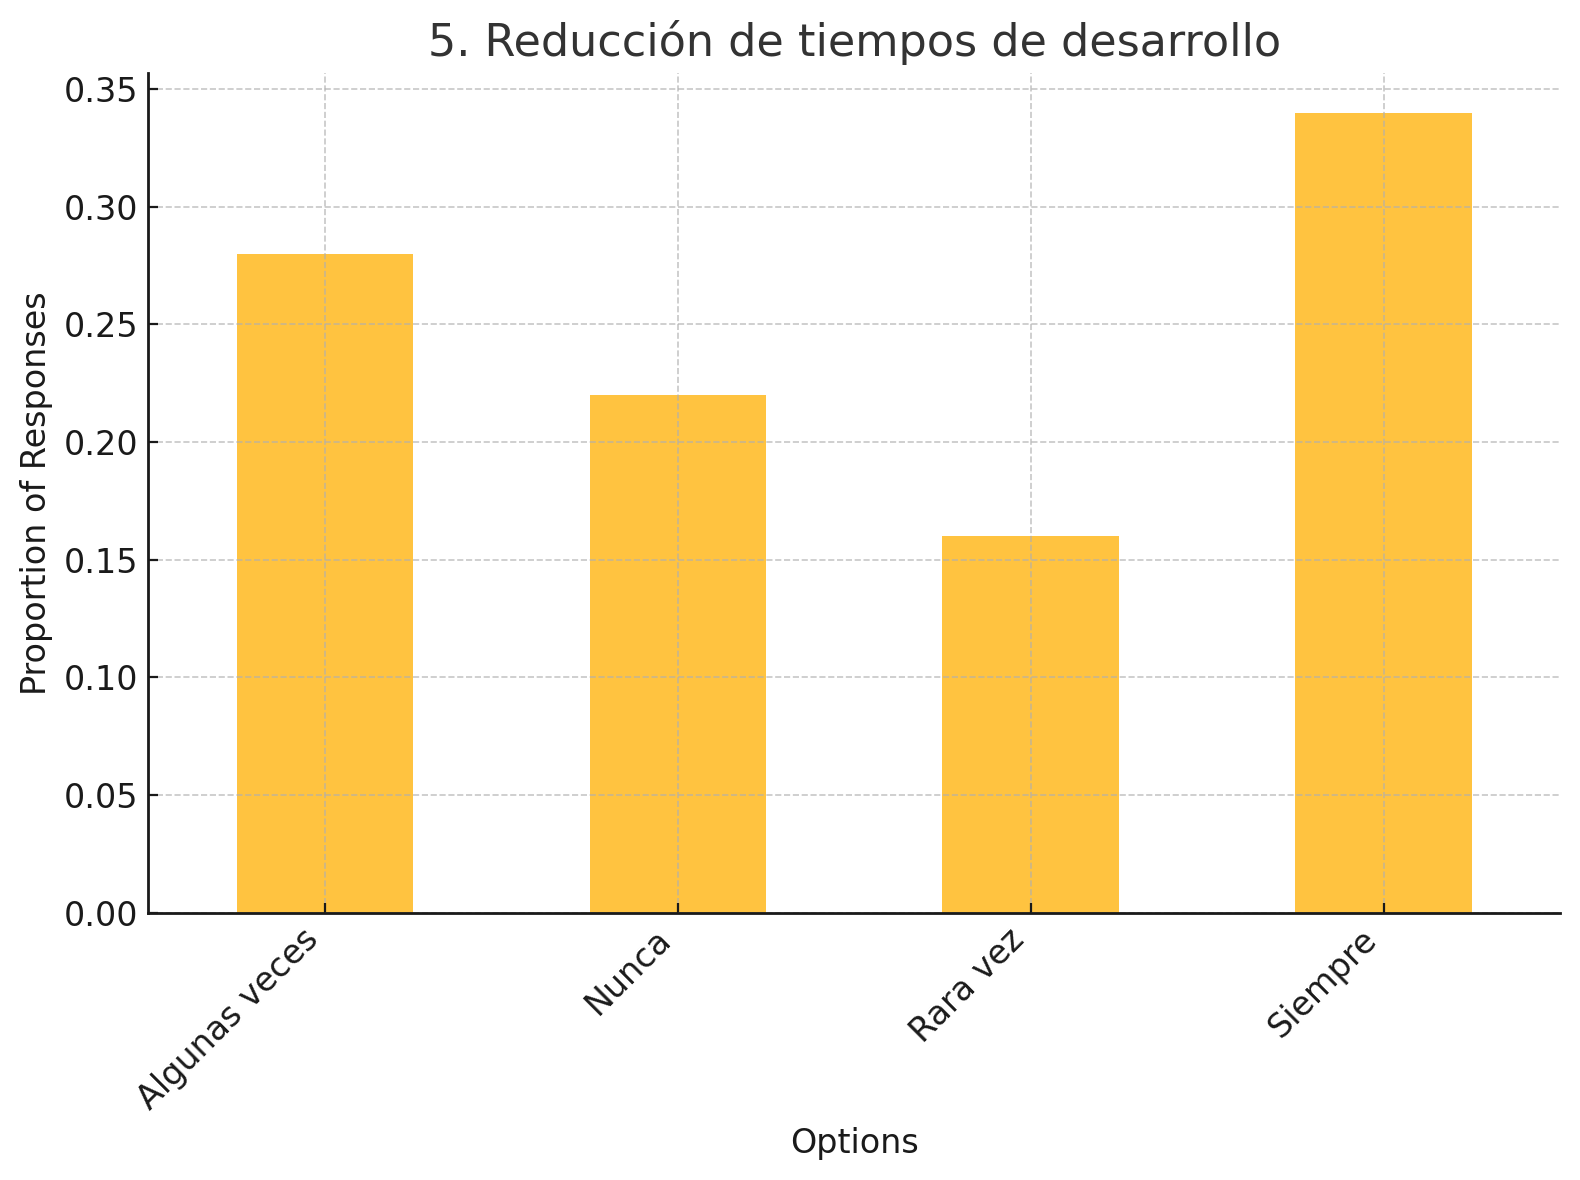
\includegraphics[width=8cm]{images/question5.png}
    \centering
\end{figure}

Conclusión: La percepción está dividida, aunque una buena proporción indica que “algunas veces” o “siempre” reducen tiempos, subrayando la eficiencia esperada de estas tecnologías.\\

\textbf{6. ¿Qué porcentaje del presupuesto de un proyecto, en promedio, se reduce
utilizando tecnologías multiplataforma?}

\begin{figure}[h!]
    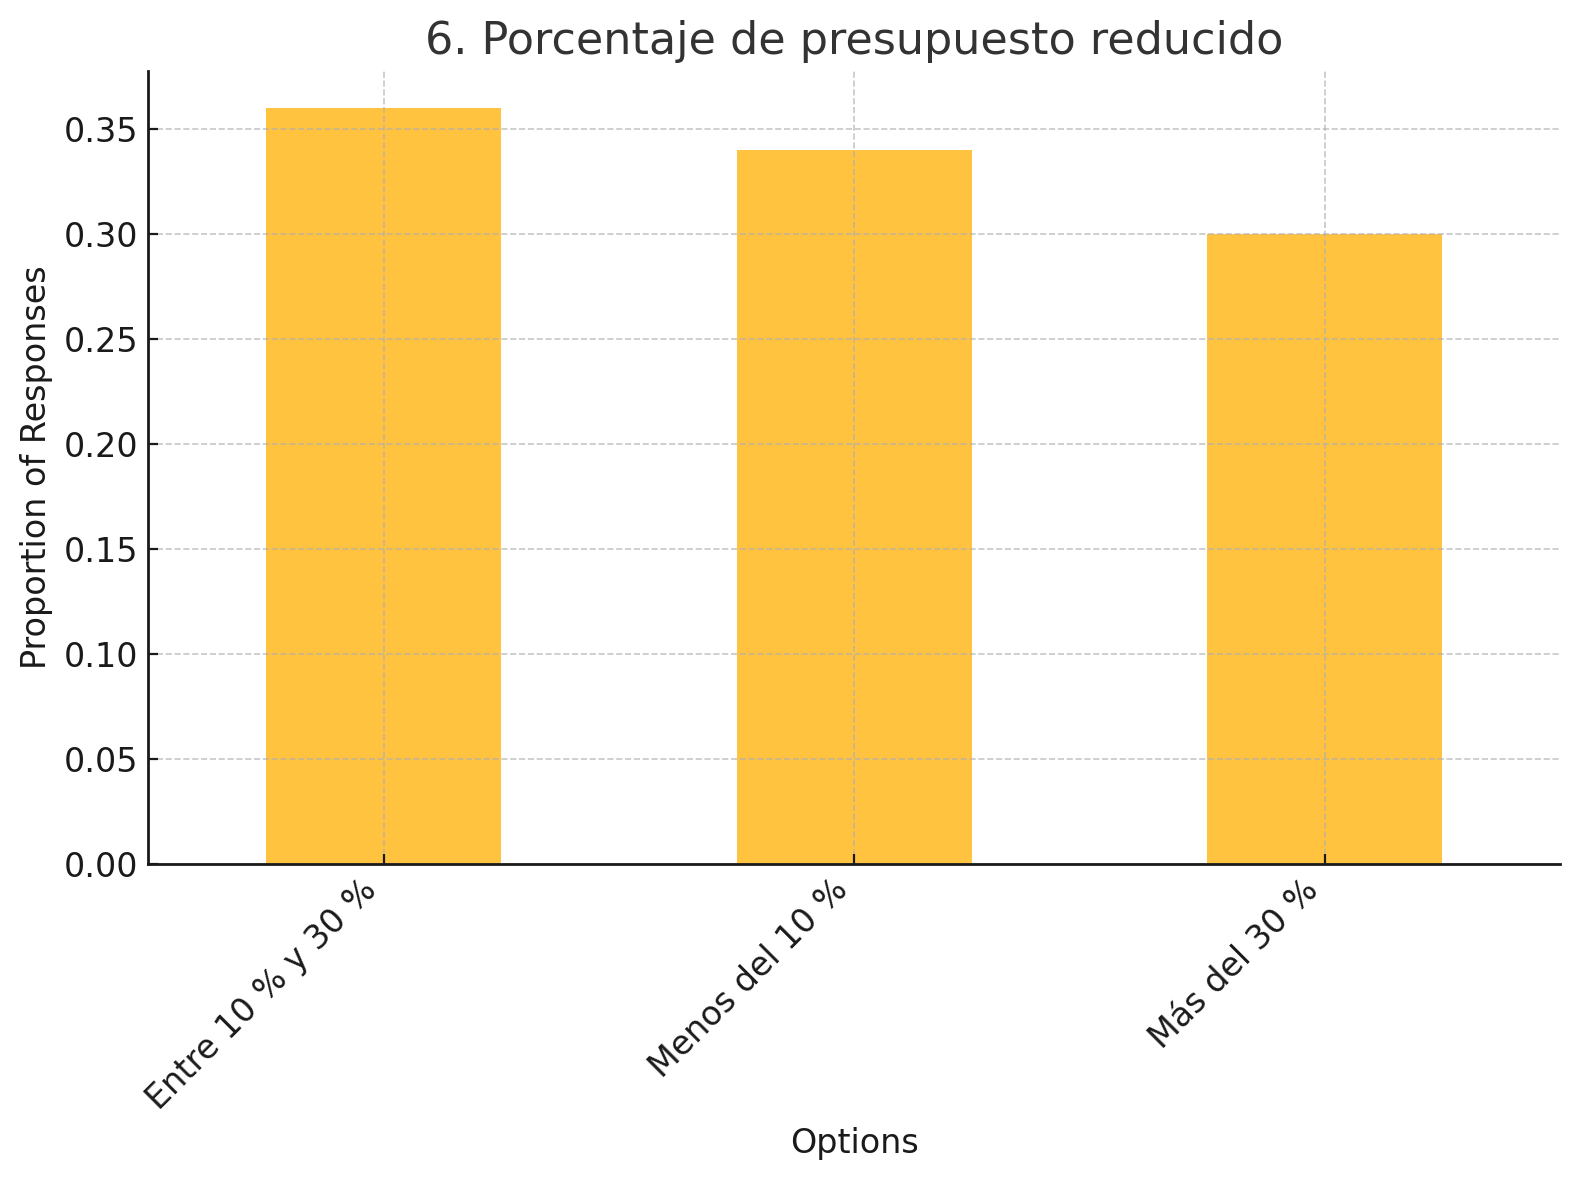
\includegraphics[width=8cm]{images/question6.png}
    \centering
\end{figure}

Conclusión: Más del 30 \% y 10-30 \% dominan, evidenciando un impacto notable en los presupuestos al usar tecnologías multiplataforma.\\

\newpage
\textbf{7. ¿Qué tan fácil es el mantenimiento de aplicaciones desarrolladas con tec-
nologías multiplataforma en comparación con las nativas?}

\begin{figure}[h!]
    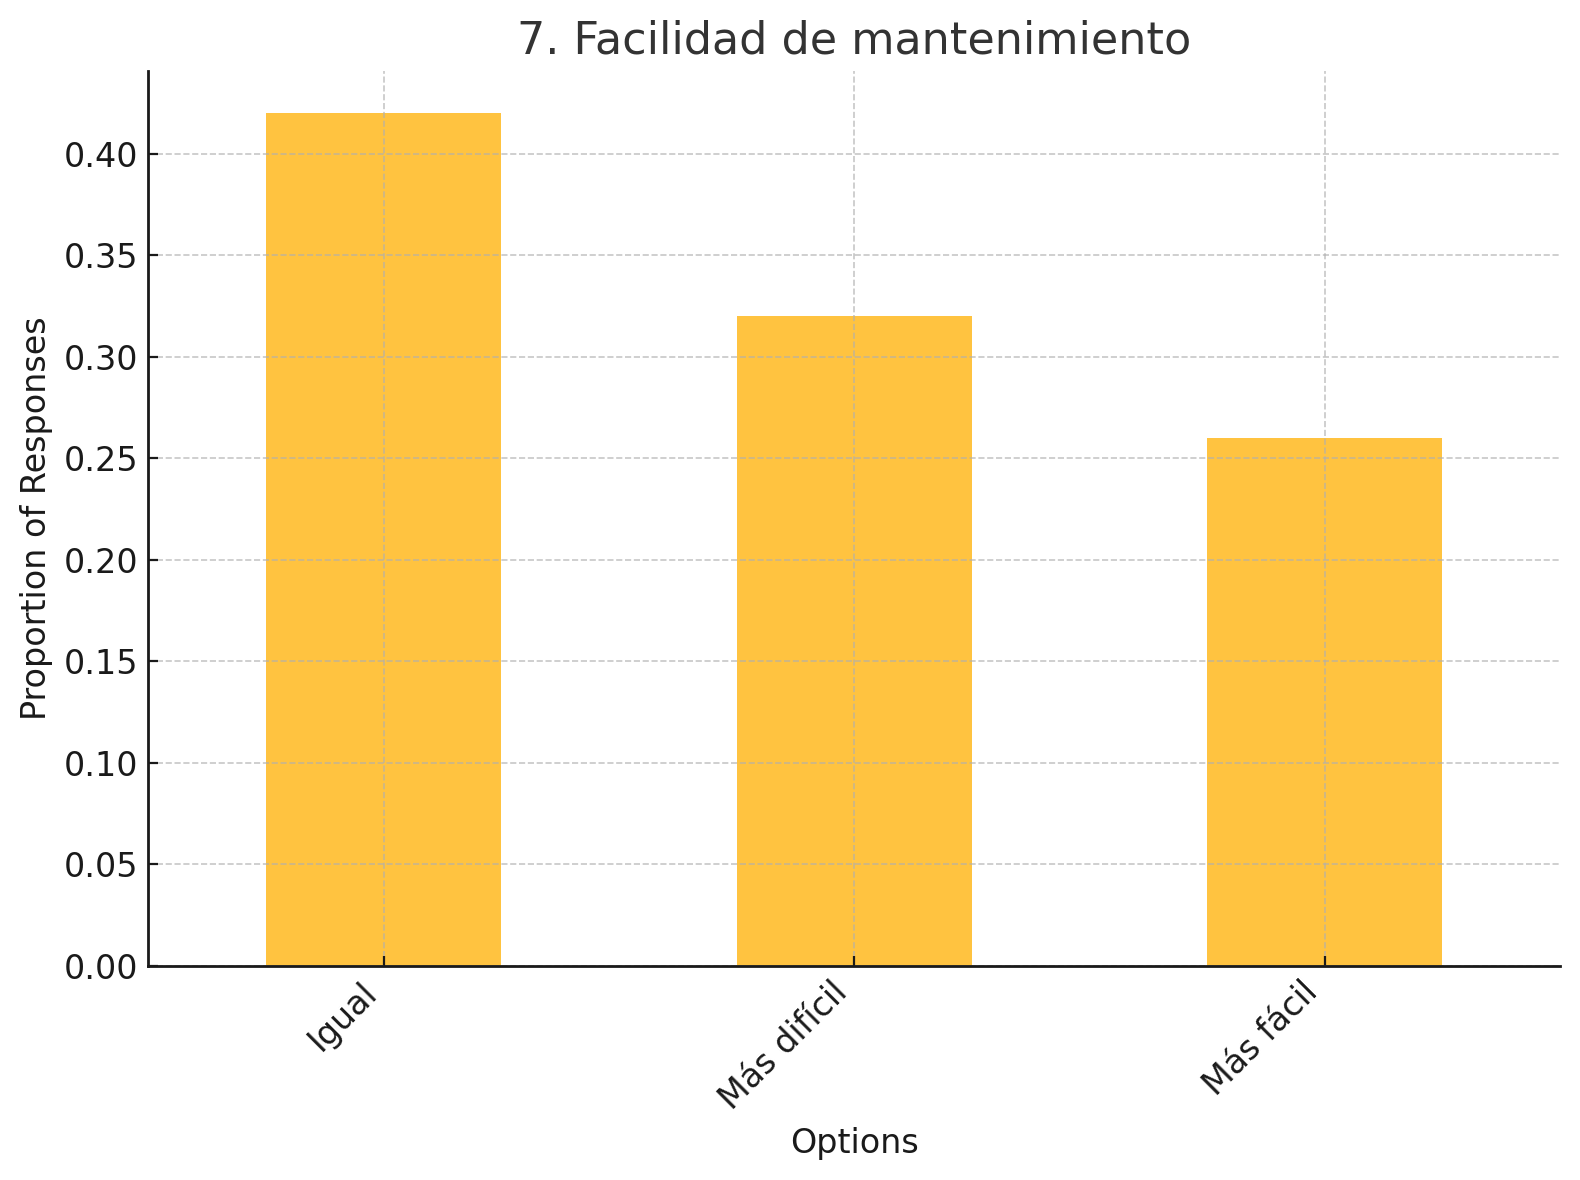
\includegraphics[width=8cm]{images/question7.png}
    \centering
\end{figure}

Conclusión: Predomina la percepción de que el mantenimiento es igual o más fácil con tecnologías multiplataforma, lo que refuerza su viabilidad en proyectos.\\

\textbf{8. En términos de calidad de la experiencia del usuario, ¿cómo califica el ren-
dimiento de las aplicaciones multiplataforma frente a las nativas?}

\begin{figure}[h!]
    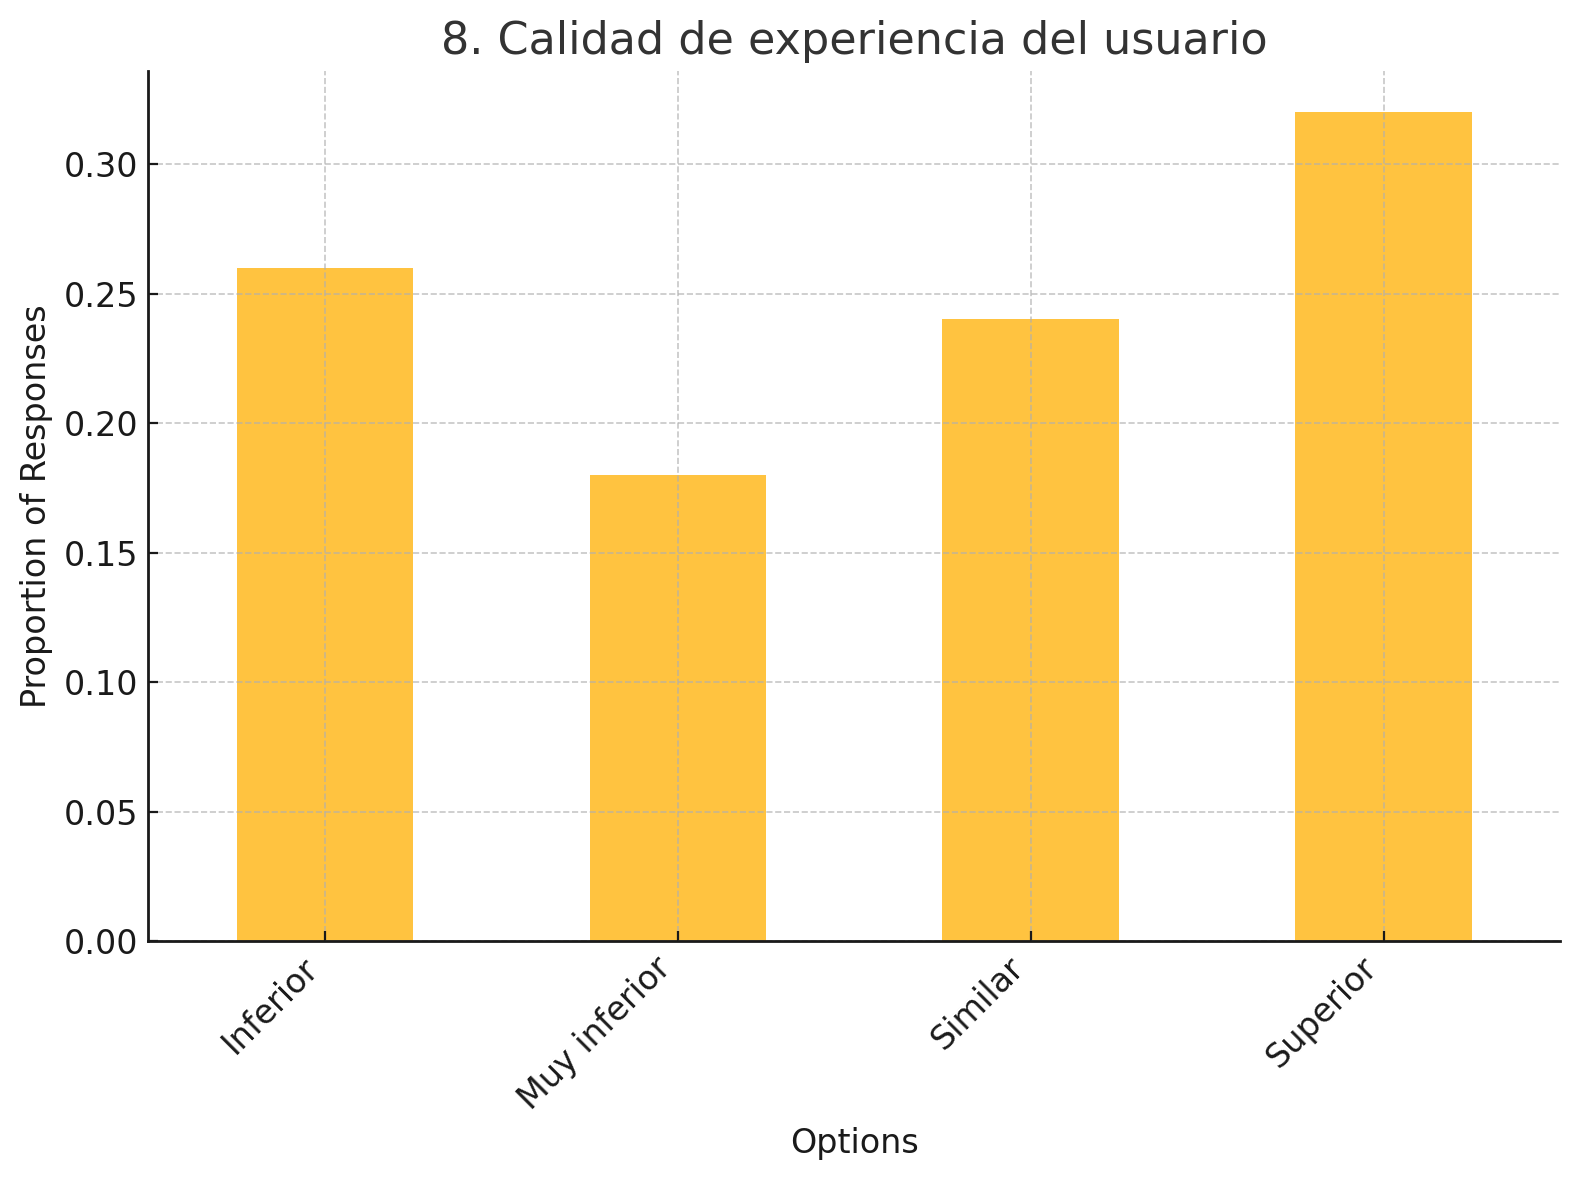
\includegraphics[width=8cm]{images/question8.png}
    \centering
\end{figure}

Conclusión: La calidad se percibe mayoritariamente como similar o superior, lo que indica que las limitaciones técnicas no afectan significativamente la experiencia del usuario.\\

\newpage
\textbf{9. ¿Qué tan frecuentemente enfrenta problemas de compatibilidad en proyec-
tos multiplataforma?}

\begin{figure}[h!]
    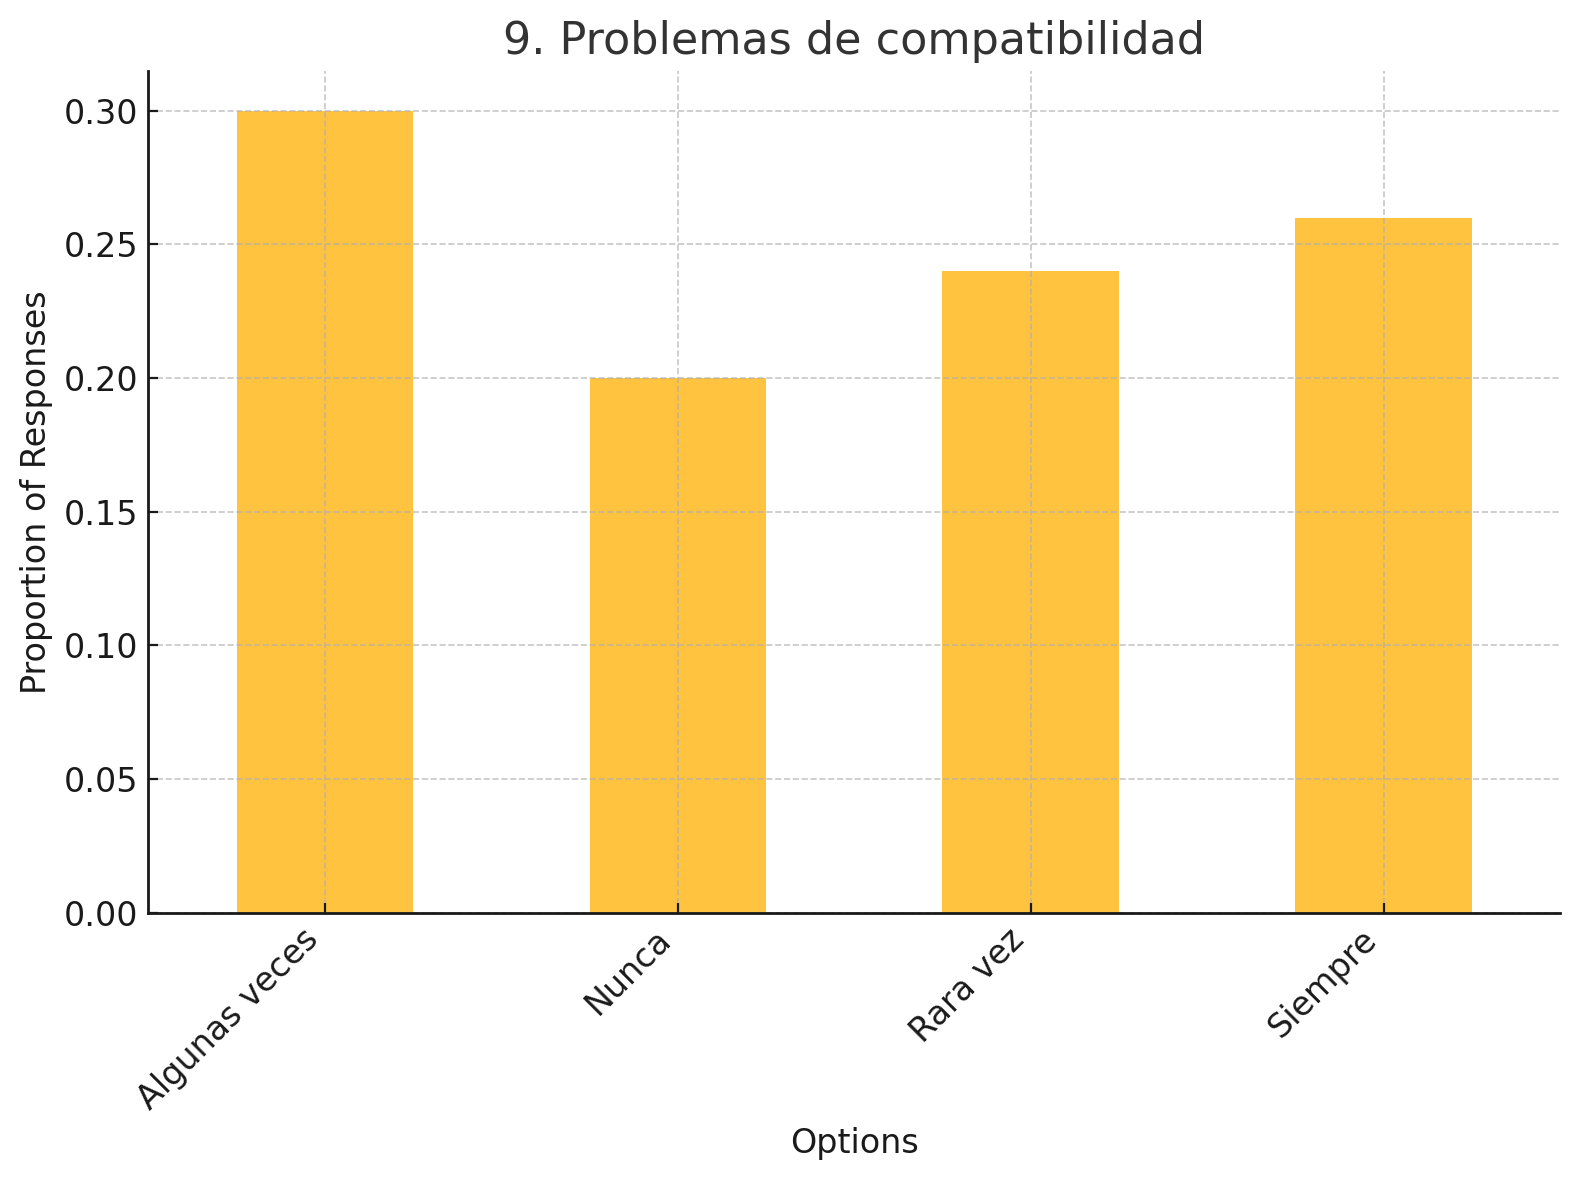
\includegraphics[width=8cm]{images/question9.png}
    \centering
\end{figure}

Conclusión: Aunque hay quienes enfrentan problemas algunas veces, la mayoría los experimenta rara vez o nunca, destacando mejoras en la compatibilidad.\\

\textbf{10. ¿Cuál es su nivel de satisfacción general con el uso de tecnologías multi-
plataforma en proyectos móviles?}

\begin{figure}[h!]
    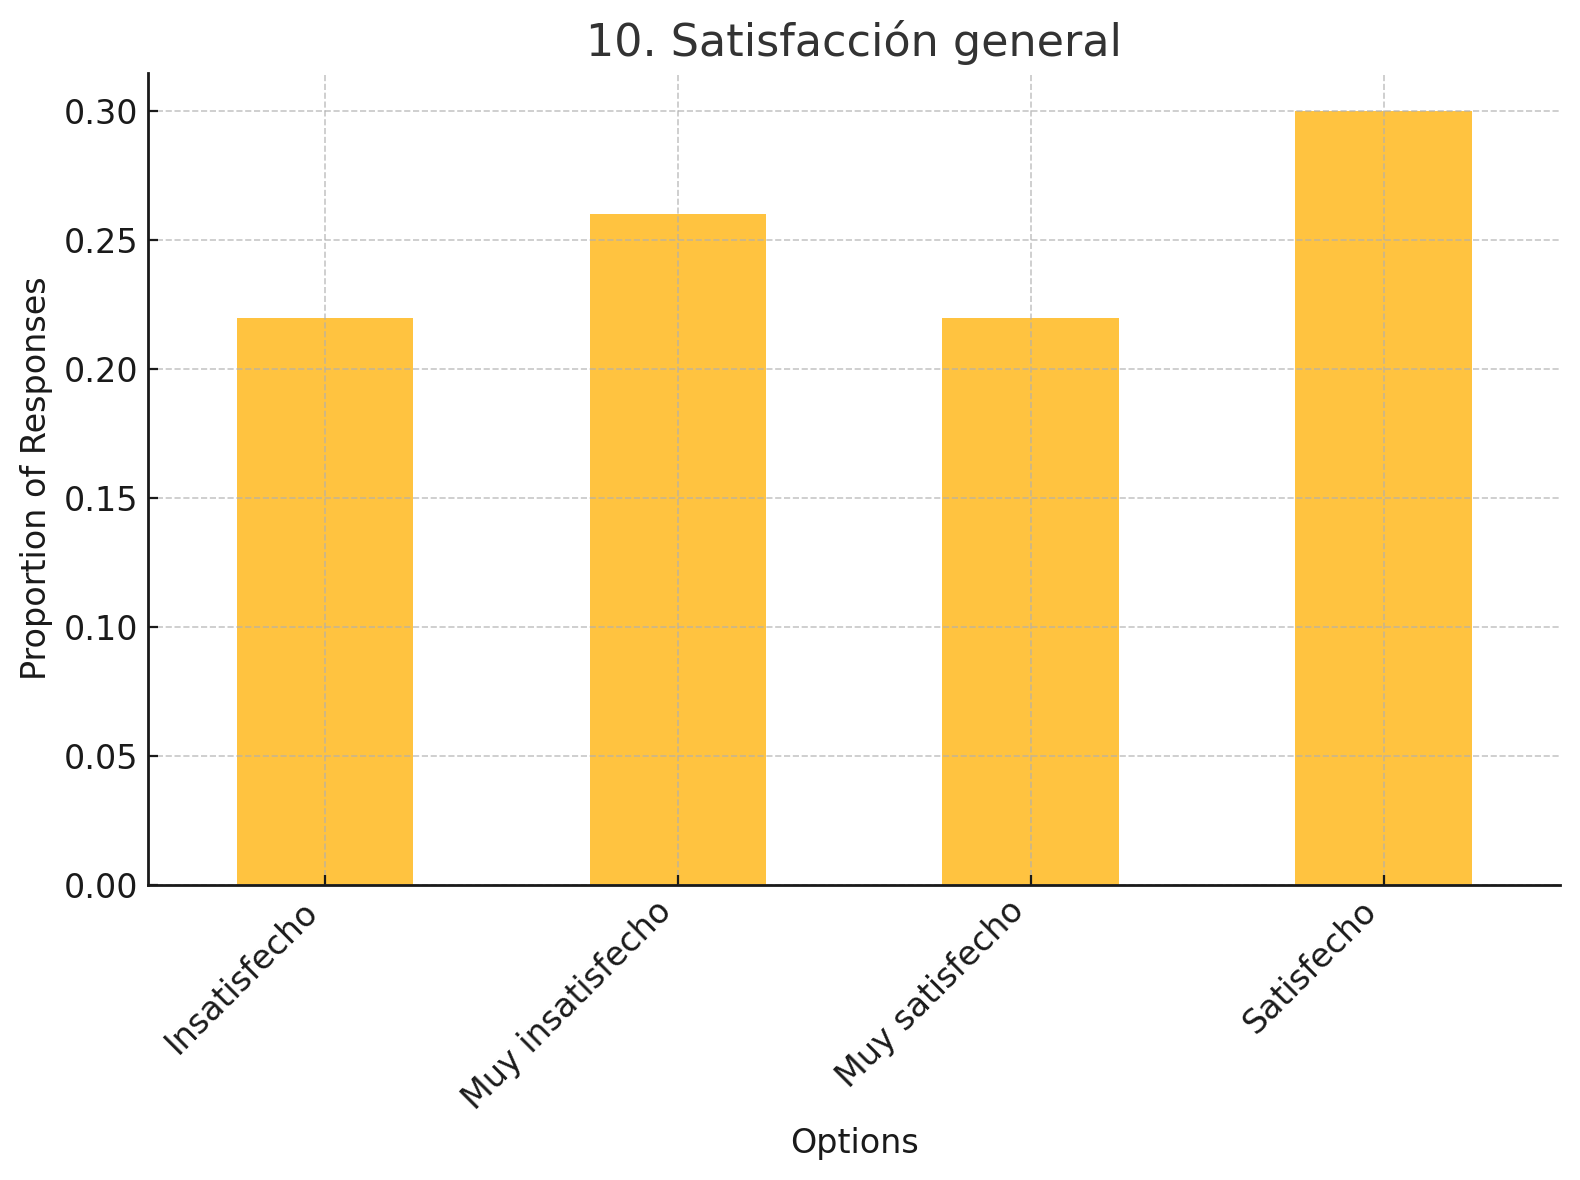
\includegraphics[width=8cm]{images/question10.png}
    \centering
\end{figure}

Conclusión: La satisfacción general es alta, con muchos encuestados indicando estar satisfechos o muy satisfechos, validando la confianza en tecnologías multiplataforma.\\

\newpage
\textbf{11. ¿Qué tan probable es que recomiende el uso de tecnologías multiplatafor-
ma para proyectos futuros?}

\begin{figure}[h!]
    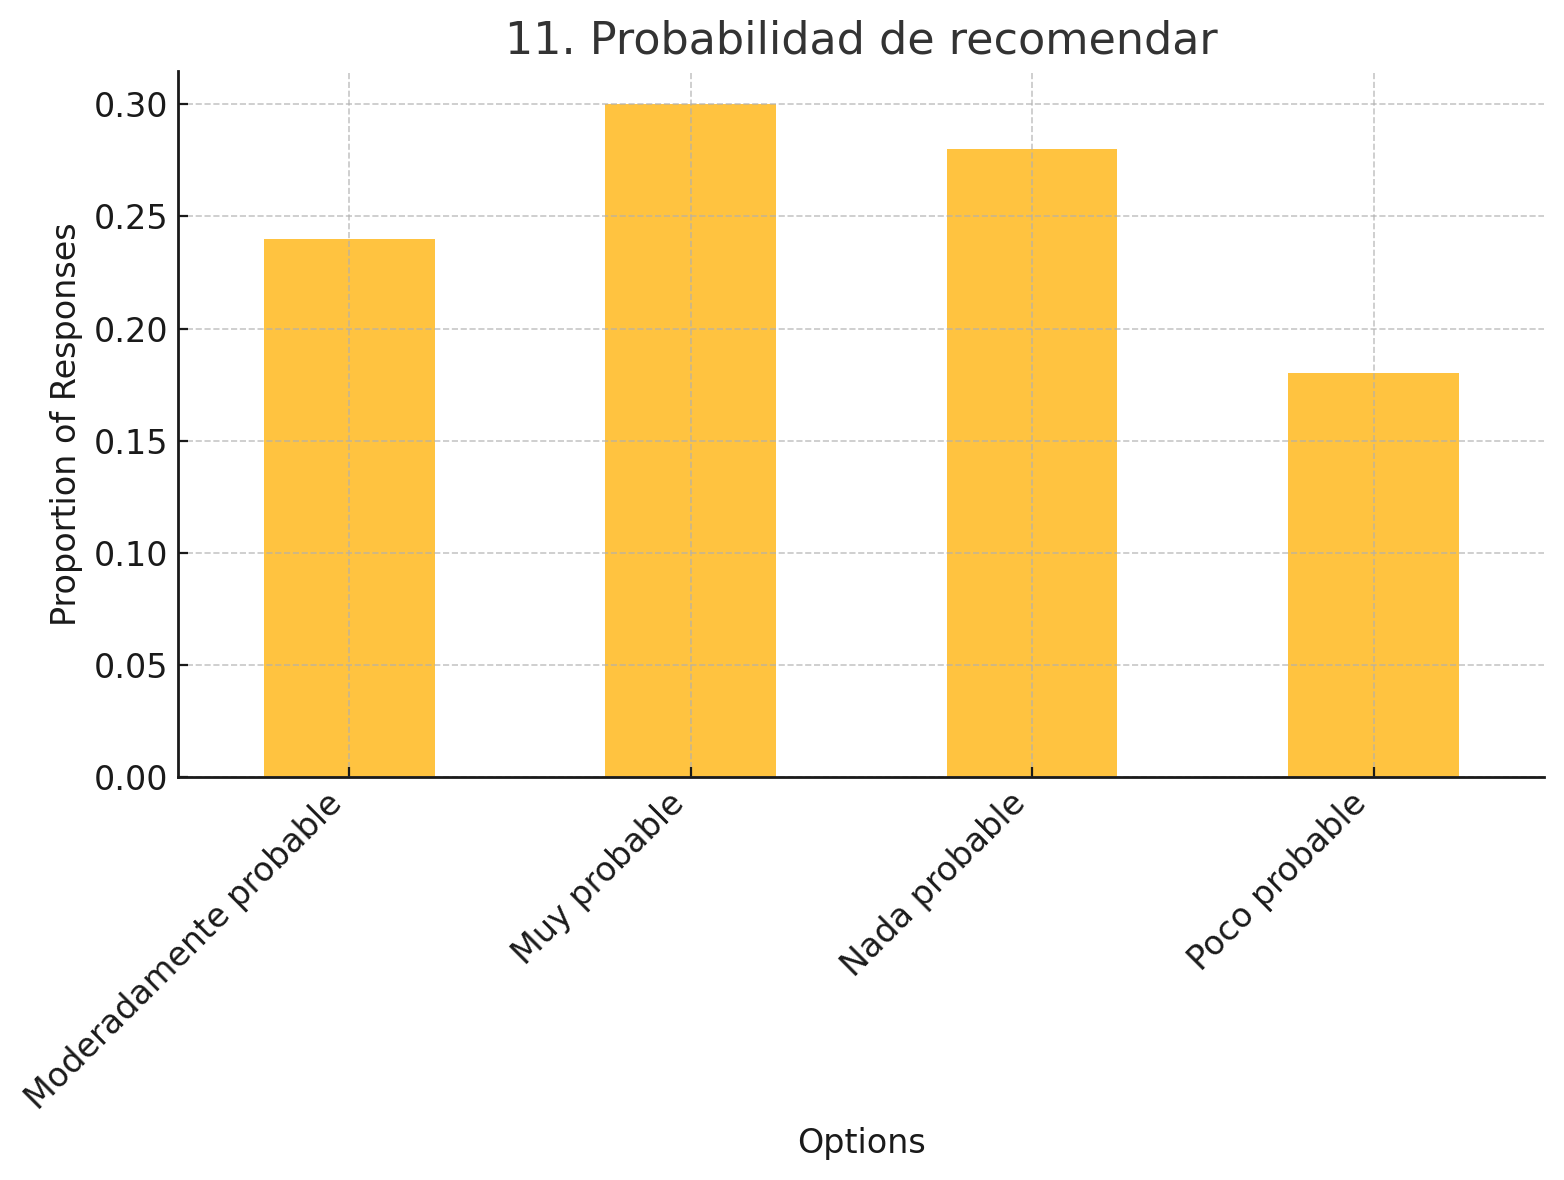
\includegraphics[width=8cm]{images/question11.png}
    \centering
\end{figure}

Conclusión: Las respuestas indican una alta probabilidad de recomendación, con muchos participantes considerando esta tecnología como moderadamente o muy probable de recomendar.\\

\textbf{12. ¿Considera que las tecnologías multiplataforma son una solución sosteni-
ble a largo plazo para el desarrollo de aplicaciones móviles?}

\begin{figure}[h!]
    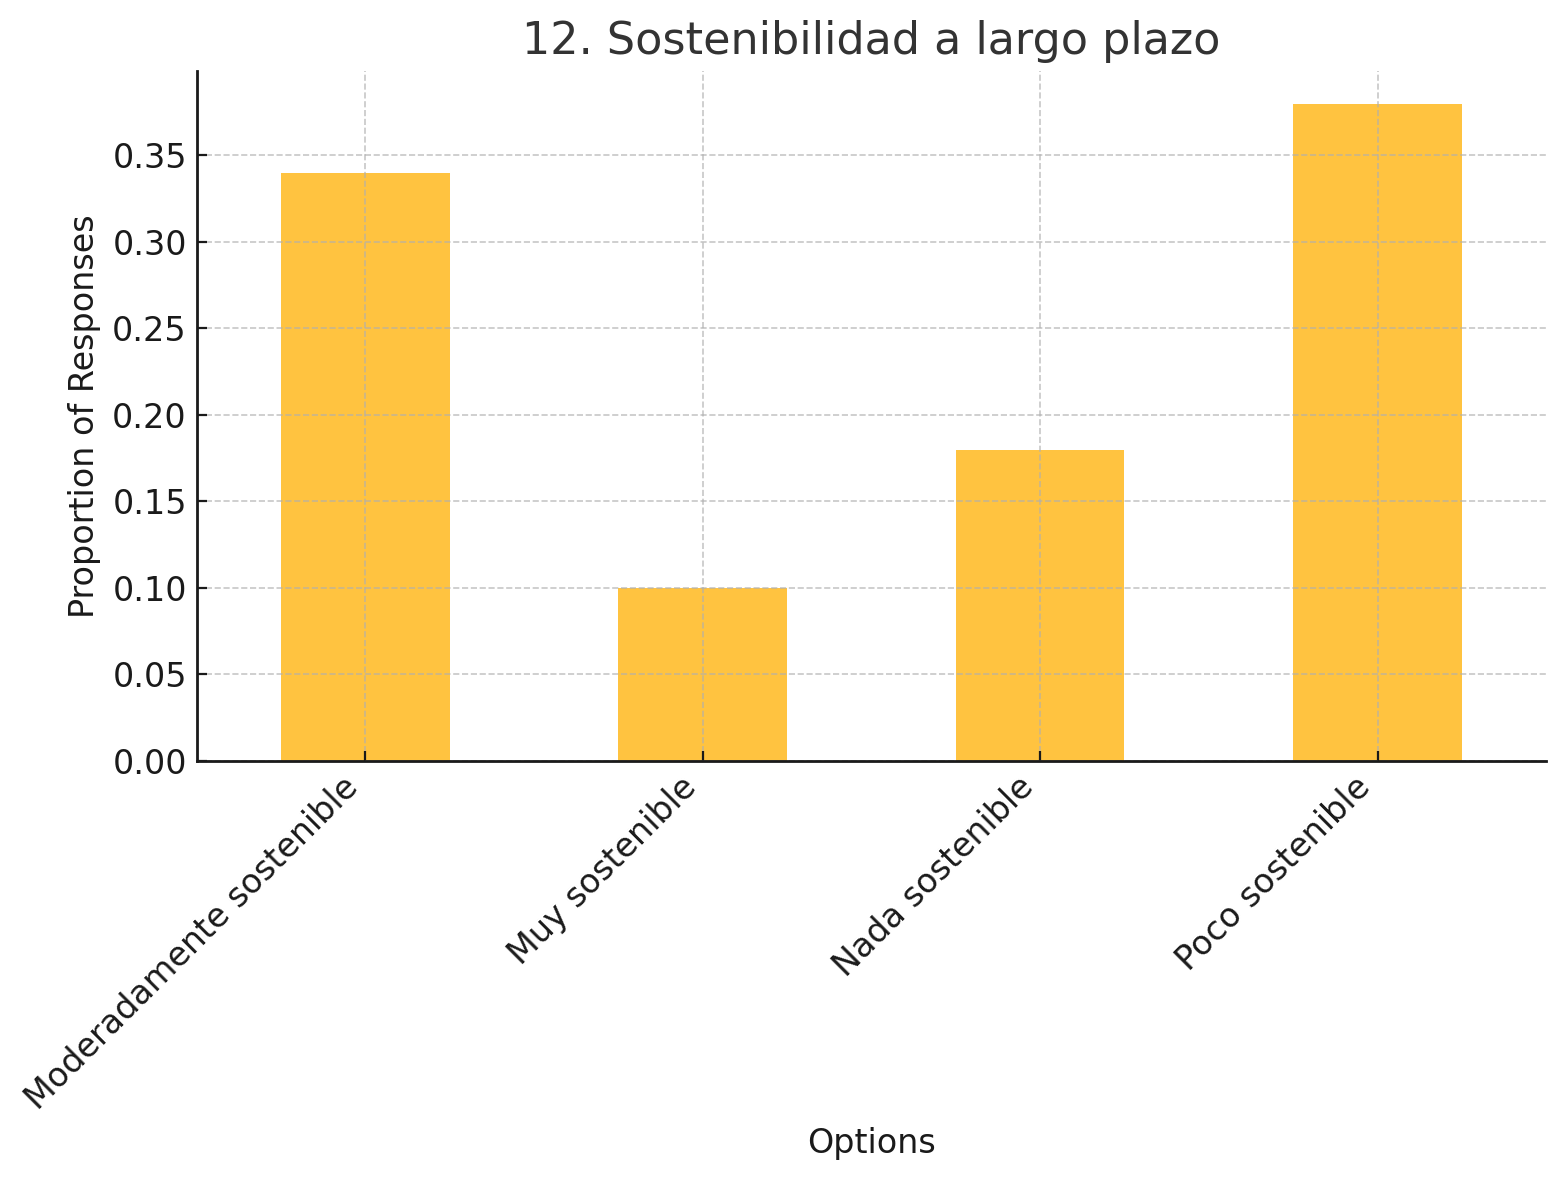
\includegraphics[width=8cm]{images/question12.png}
    \centering
\end{figure}

Conclusión: La mayoría considera que las tecnologías multiplataforma son moderadamente o muy sostenibles, destacando su potencial como solución a largo plazo.

\newpage
\subsection{Conclusiones generales}

La programación multiplataforma se caracteriza por su enfoque en reutilizar código para múltiples sistemas operativos, reduciendo redundancias. Frameworks como Flutter, React Native y Xamarin son ampliamente adoptados debido a su flexibilidad, soporte robusto y facilidad de integración, ofreciendo una alternativa viable a los entornos nativos.\\

El desarrollo multiplataforma tiende a reducir los costos al minimizar la duplicación de esfuerzos para múltiples plataformas. Sin embargo, los costos iniciales de aprendizaje, herramientas específicas y la necesidad de optimizaciones técnicas pueden influir en la relación costo-beneficio, especialmente en proyectos complejos.\\

Aunque las aplicaciones nativas ofrecen un rendimiento óptimo y acceso total a las capacidades del dispositivo, las multiplataforma han mejorado significativamente, ofreciendo una experiencia de usuario comparable y funcionalidad suficiente para la mayoría de los casos, salvo en aplicaciones que exigen máxima precisión o personalización.\\

El desarrollo multiplataforma permite ahorros sustanciales de tiempo y costos al compartir código entre plataformas, especialmente en proyectos con recursos limitados. Además, el mantenimiento es más eficiente al centralizar las actualizaciones en una base de código única, lo que lo hace una opción práctica para empresas pequeñas y medianas.\\

Se recomienda adoptar frameworks multiplataforma como Flutter o React Native para proyectos con requerimientos generales, priorizando evaluaciones iniciales de necesidades específicas. Las empresas con recursos limitados deben enfocarse en proyectos con menor complejidad nativa y aprovechar las comunidades y recursos gratuitos disponibles para formación y soporte.\\
\newpage
\section{Recomendaciones}

\textbf{1. Selecciona el framework adecuado según las necesidades del proyecto}

Antes de optar por una solución multiplataforma, evalúa los requerimientos técnicos y funcionales del proyecto. Frameworks como Flutter son ideales para aplicaciones con interfaces complejas y animaciones fluidas, mientras que React Native ofrece mayor flexibilidad para integraciones nativas. Realiza pruebas piloto para validar el desempeño del framework elegido en escenarios reales.
	
\textbf{2. Prioriza proyectos con requisitos generales y menor dependencia nativa}

La programación multiplataforma es más efectiva en aplicaciones que no necesitan un acceso intensivo a funciones específicas del hardware, como gráficos avanzados, procesamiento intensivo o personalización a nivel del sistema operativo. Si el proyecto implica funcionalidades altamente especializadas, considera combinar desarrollo nativo con soluciones multiplataforma (aproximación híbrida).
	
\textbf{3.	Capacita al equipo en el uso de tecnologías multiplataforma}

Invierte en la formación del equipo de desarrollo para que dominen los frameworks multiplataforma y sus mejores prácticas. Esto incluye aprovechar comunidades activas, tutoriales oficiales y recursos de aprendizaje. Además, fomenta el uso de patrones de diseño reutilizables que faciliten la escalabilidad y el mantenimiento a largo plazo.
	
\textbf{4.	Planifica pruebas de compatibilidad y mantenimiento desde el inicio}

Aunque la multiplataforma permite compartir la mayor parte del código, los problemas de compatibilidad entre dispositivos y sistemas operativos pueden surgir. Implementa pruebas tempranas en diferentes entornos y dispositivos para garantizar una experiencia uniforme. Asimismo, aprovecha la centralización del código para agilizar las actualizaciones y reducir costos de mantenimiento.

\newpage
\printbibliography

\appendix
\newpage
\section{Anexos}
\subsection{Encuesta}

\textbf{Encuesta : } Uso de tecnologías multiplataforma en el desarrollo de aplicaciones móviles.\\

\textbf{Instrucciones : }  Por favor, lea detenidamente cada pregunta y marque la opción que mejor
refleje su experiencia y opinión. Sus respuestas serán confidenciales y utilizadas exclusivamente para fines académicos.

\subsection*{Sección 1: Datos generales}

\noindent
1. ¿Cuál es su cargo en la startup?  
   \begin{itemize}
       \item[a)] Tech Lead  
       \item[b)] Desarrollador Senior  
   \end{itemize}

\noindent
2. ¿Cuántos años de experiencia tiene en el desarrollo de aplicaciones móviles?  
   \begin{itemize}
       \item[a)] Menos de 3 años  
       \item[b)] 3-5 años  
       \item[c)] Más de 5 años  
   \end{itemize}

\noindent
3. ¿Qué tipo de tecnologías utiliza principalmente en su trabajo?  
   \begin{itemize}
       \item[a)] Tecnologías nativas  
       \item[b)] Tecnologías multiplataforma  
       \item[c)] Ambas  
   \end{itemize}

\subsection*{Sección 2: Costos y tiempo de desarrollo}

\noindent
4. ¿En qué medida considera que las tecnologías multiplataforma reducen los costos de desarrollo en comparación con las tecnologías nativas?  
   \begin{itemize}
       \item[a)] Nada  
       \item[b)] Poco  
       \item[c)] Moderadamente  
       \item[d)] Mucho  
   \end{itemize}

\noindent
5. Según su experiencia, ¿las tecnologías multiplataforma permiten acortar los tiempos de desarrollo?  
   \begin{itemize}
       \item[a)] Nunca  
       \item[b)] Rara vez  
       \item[c)] Algunas veces  
       \item[d)] Siempre  
   \end{itemize}

\noindent
6. ¿Qué porcentaje del presupuesto de un proyecto, en promedio, se reduce utilizando tecnologías multiplataforma?  
   \begin{itemize}
       \item[a)] Menos del 10\%  
       \item[b)] Entre 10\% y 30\%  
       \item[c)] Más del 30\%  
   \end{itemize}

\subsection*{Sección 3: Facilidad de mantenimiento y experiencia del usuario}

\noindent
7. ¿Qué tan fácil es el mantenimiento de aplicaciones desarrolladas con tecnologías multiplataforma en comparación con las nativas?  
   \begin{itemize}
       \item[a)] Más difícil  
       \item[b)] Igual  
       \item[c)] Más fácil  
   \end{itemize}

\noindent
8. En términos de calidad de la experiencia del usuario, ¿cómo califica el rendimiento de las aplicaciones multiplataforma frente a las nativas?  
   \begin{itemize}
       \item[a)] Muy inferior  
       \item[b)] Inferior  
       \item[c)] Similar  
       \item[d)] Superior  
   \end{itemize}

\noindent
9. ¿Qué tan frecuentemente enfrenta problemas de compatibilidad en proyectos multiplataforma?  
   \begin{itemize}
       \item[a)] Nunca  
       \item[b)] Rara vez  
       \item[c)] Algunas veces  
       \item[d)] Siempre  
   \end{itemize}

\subsection*{Sección 4: Percepción y preferencia}

\noindent
10. ¿Cuál es su nivel de satisfacción general con el uso de tecnologías multiplataforma en proyectos móviles?  
    \begin{itemize}
        \item[a)] Muy insatisfecho  
        \item[b)] Insatisfecho  
        \item[c)] Satisfecho  
        \item[d)] Muy satisfecho  
    \end{itemize}

\noindent
11. ¿Qué tan probable es que recomiende el uso de tecnologías multiplataforma para proyectos futuros?  
    \begin{itemize}
        \item[a)] Nada probable  
        \item[b)] Poco probable  
        \item[c)] Moderadamente probable  
        \item[d)] Muy probable  
    \end{itemize}

\noindent
12. ¿Considera que las tecnologías multiplataforma son una solución sostenible a largo plazo para el desarrollo de aplicaciones móviles?  
    \begin{itemize}
        \item[a)] Nada sostenible  
        \item[b)] Poco sostenible  
        \item[c)] Moderadamente sostenible  
        \item[d)] Muy sostenible  
    \end{itemize}

\textbf{Agradecimiento : } Agradecemos su tiempo y honestidad al completar esta encuesta. Sus respuestas serán fundamentales para el análisis y las conclusiones del estudio.



\end{document}
